\documentclass{emulateapj}
\submitted{{\it Submitted for publication in ApJ}}
\usepackage{multirow,color,wrapfig,ulem}
\usepackage {graphicx}
\usepackage{graphics}
\usepackage[dvips]{epsfig}
\newcommand{\avg}[1]{\langle{#1}\rangle}  
\newcommand{\nscatt}{\langle N_{\rm  scatt}\rangle}
\newcommand{\ly}{{\ifmmode{{\rm Ly}\alpha~}\else{Ly$\alpha$~}\fi}}
\newcommand{\hMpc}{{\ifmmode{h^{-1}{\rm Mpc}}\else{$h^{-1}$Mpc }\fi}}   
\newcommand{\hGpc}{{\ifmmode{h^{-1}{\rm Gpc}}\else{$h^{-1}$Gpc }\fi}}   
\newcommand{\hmpc}{{\ifmmode{h^{-1}{\rm Mpc}}\else{$h^{-1}$Mpc }\fi}}  
\newcommand{\hkpc}{{\ifmmode{h^{-1}{\rm kpc}}\else{$h^{-1}$kpc }\fi}}  
\newcommand{\hMsun}{{\ifmmode{h^{-1}{\rm
        {M_{\odot}}}}\else{$h^{-1}{\rm{M_{\odot}}}$}\fi}}   
\newcommand{\hmsun}{{\ifmmode{h^{-1}{\rm
        {M_{\odot}}}}\else{$h^{-1}{\rm{M_{\odot}}}$}\fi}}   
\newcommand{\Msun}{{\ifmmode{{\rm {M_{\odot}}}}\else{${\rm{M_{\odot}}}$}\fi}}  
\newcommand{\msun}{{\ifmmode{{\rm {M_{\odot}}}}\else{${\rm{M_{\odot}}}$}\fi}}  
\newcommand{\lya}{{Lyman $\alpha$~}}
\newcommand{\clara}{{\texttt{CLARA}}~}
\newcommand{\rand}{{\ifmmode{{\mathcal{R}}}\else{${\mathcal{R}}$ }\fi}}  
\newcommand{\hs}{{\hspace{1mm}}}  
\newcommand{\kms}{{\ifmmode{{\mathrm{\,km\ s}^{-1}}}\else{\,km~s$^{-1}$}\fi}}

% definition to produce a "less than or similar to" symbol
\def\lsim{~\rlap{$<$}{\lower 1.0ex\hbox{$\sim$}}}

% definition to produce a "greater than or similar to" symbol
\def\gsim{~\rlap{$>$}{\lower 1.0ex\hbox{$\sim$}}}

\begin{document}

\title{The impact of gas bulk rotation on the Lyman $\alpha$ line} 
\shorttitle{Rotation effects on the Lyman $\alpha$ line}

\shortauthors{Garavito-Camargo, Forero-Romero \& Dijkstra}

\author{ Juan N. Garavito-Camargo, Jaime E. Forero-Romero}
\affil{Departamento de F\'{i}sica, Universidad de los Andes, Cra. 1
No. 18A-10, Edificio Ip, Bogot\'a, Colombia}
\email{jn.garavito57@uniandes.edu.co}
\email{je.forero@uniandes.edu.co}
\and
\author{Mark Dijkstra}
\affil{Institute of Theoretical Astrophysics, University of Oslo,
  Postboks 1029, 0858 Oslo, Norway} 
\email{mark.dijkstra@astro.uio.no }

\keywords{galaxies: high-redshift --- line: formation --- methods:
  numerical ---  radiative transfer} 
\begin{abstract}

We present results of radiative transfer calculations to measure the
impact of gas bulk rotation on the morphology of the Lyman $\alpha$
emission line in distant galaxies. We model a galaxy as a sphere with
an homogeneous mixture of dust and hydrogen at a constant
temperature. These spheres have a solid-body rotation with maximum
velocities in the range $0-300$ \kms and neutral hydrogen optical
depths in the range $\tau_{\rm H}=10^{5}-10^{7}$. We consider cases 
of a single central \lya source, and a uniform distribution of sources. 
Our main result is that rotation introduces a dependence of the
line morphology with  viewing angle. Observations parallel to the
rotation axis yield lines similar to the static case. The greatest
difference is observed perpendicular to the rotation axis where the
intensity at the line center increases with rotational velocity.  For
homogeneously distributed sources the line becomes single peaked  at
rotational velocities larger than half the line width in the static
case. However, rotation does not not induce any significant anisotropy
in the total line intensity or in the escape fraction. 
\end{abstract}



\section{Introduction}
\label{sec:intro}

The detection of strong \ly emission lines has become an essential
method in extra-galactic astronomy to find distant star-forming
galaxies
\citep{PartridgePeebles,Rhoads00,Gawiser2007,Koehler2007,Ouchi08,Yamada2012,Schenker2012,Finkelstein2013}.
The galaxies detected using this method receive the 
name of \ly emitters (LAEs). A detailed examination of this galaxy
population has diverse implications for galaxy formation, reionization
and the large scale structure of the Universe. Attempts to fully
exploit the physical information included in the \ly line require an
understanding of all the physical factors involved in shaping the
line. Due to the resonant nature of this line, these physical factors
notably include temperature, density and bulk velocity field of the neutral
Hydrogen in the emitting galaxy and its surroundings.


A basic understanding of the quantitative behavior of the \ly line
has been reached through analytic studies in the case of a static
configurations, such as uniform slabs
\citep{Adams72,Harrington73,Neufeld90} and uniform spheres
\citep{Dijkstra06}. Analytic studies of configurations including
some kind of bulk flow only include the case of a sphere with a Hubble
like expansion flow \citep{LoebRybicki}. 

A quantitative description of the \ly line has been reached through
Monte Carlo simulations \citep{Auer68,Avery68,Adams72}. In the last
two decades these studies have become popular due to the
availability of computing power. Early into the 21st century, the first
studies focused on homogeneous and static media
\citep{Ahn00,Ahn01,Zheng02}. Later on, the effects of clumpy media
\citep{Hansen06} and expanding/contracting shell/spherical geometries started to
be studied \citep{Verhamme06,Dijkstra06,Ahn2014}. Similar codes have applied
these results to semi-analytic models of galaxy formation \citep{Orsi12, Garel2012} and
results of large hydrodynamic simulations
\citep{CLARA,Forero12,Behrens13}. Recently, Monte Carlo codes have also
been applied to the results of high resolution hydrodynamic
simulations of individual
galaxies \citep{Laursen09,Barnes11,Verhamme12,Yajima12}. Meanwhile, recent
developments have been focused on the systematic study of clumpy
outflows \citep{DijkstraKramer}and anisotropic velocity configurations
\citep{Zheng2013}. 

The recent studies of galaxies in hydrodynamic simulations
\citep{Laursen09,Barnes11,Verhamme12,Yajima12} have all shown
systematic variations in the \ly line with the viewing angle. These
variations are a complex superposition of anisotropic density
configurations (i.e. edge-on vs. face-on view of a galaxy), the
inflows observed by gas cooling and the outflows included in the
supernova feedback process of the simulation. These bulk flows
physically correspond to the circumgalactic and intergalactic medium
(CGM and IGM). These effects are starting to be studied
 in simplified configurations that vary the density and wind
 characteristics \citep{Zheng2013,Behrens2014}. 

However, in all these efforts the effect of rotation,
which is an ubiquitous feature in galaxies, has not been
systematically studied. The processing of the \ly photons in a
rotating interstellar medium (ISM) must have some kind of impact in
the \ly line morphology. 

Performing that study is the main goal of this paper. We investigate for the
first time the impact of rotation on the morphology of the \ly
line. We focus on a simplified system: a spherical gas cloud with
homogeneous density and solid body rotation, to study the line
morphology and the escape fraction in the presence of dust. We base
our work on two independent Monte Carlo based radiative transfer codes
presented in \cite{CLARA} and \cite{DijkstraKramer}.   
  
This paper is structured as follows: In \S \ref{sec:implementation} we
present the implementation of bulk rotation into the Monte Carlo
codes, paying special attention to coordinate definitions. We also
present a short review of how the \ly radiative transfer codes work
and list the different physical parameters in the simulated grid of
models. In \S \ref{sec:results} we present the results of the
simulations, with special detail to quantities that show a
clear evolution as a function of the sphere rotational velocity. In \S
\ref{sec:discussion} we discuss the implications of our results in the
interpretation of LAEs observations with high resolution
spectroscopy. In the last section we present our conclusions.    


In this paper we express a photon's frequency in terms of the
dimensionless variable $x\equiv (\nu -\nu_a)/\Delta\nu_\alpha$, where
$\nu_{\alpha}=2.46\times 10^{15}$ Hz is the Ly$\alpha$ resonance
frequency,  $\Delta\nu_{\alpha} \equiv
\nu_{\alpha}\sqrt{2kT/m_pc^2}\equiv \nu_av_{\rm th}/c $ is the Doppler
broadening of the line which depends on the neutral gas temperature
$T$ scattering the radiation or equivalently the thermal velocity
$v_{\rm th}$ of the atoms.  For the temperature $T=10^4$K used in our
radiative transfer calculations the thermal velocity is
$v_{\rm th}=12.8$\kms.  




\section{Models of bulk gas rotation}
\label{sec:implementation}

Describing the kinematics of gas rotation in all generality is a
complex task, specially at high redshift where there is still missing
a thorough observational account of rotation in galaxies beyond
$z>1.0$. Even at low redshifts there is a great
variation in the shape of the rotation curve as observed in HI
emission as a function of the distance to the galaxy center. However
there are two recurrent features. First, in the
central galactic region the velocity increases proportional to the radius,
following a solid rotation behavior. Second, beyond a certain radius
the rotation curve tends to flatten.  An ab-initio description of
such realistic rotation curves in simulations depends on having access to
the dynamic evolution of all mass components in the galaxy: stars, gas
and dark matter. Such level of realism is extremely complex to
achieve, specially if one wants to get a systematic description based
on statistics of simulated objects. 

Following the tradition of studies of \ly emitting systems,
we implement a model with simplified geometry. We assume that the gas
is homogeneously distributed in a sphere that rotates as a solid body
with constant angular velocity. This simple model will contain only
one free parameter: the linear velocity at the sphere's surface, $V_{\rm
  max}$. 

\subsection{Detailed Implementation of Rotation}

 In the Monte Carlo code we define a Cartesian coordinate system to
 describe the position of each photon. The origin of this system
 coincides with the center of the sphere and the rotation axis is defined
 to be $z$-axis. With this choice, the components of the gas bulk velocity
 field, $\vec{v} = v_{x}\hat{i} + v_{y}\hat{j} + v_{z}\hat{k}$, can be
 written as  
  
\begin{equation}
    v_{x}=-\frac{y}{R}V_{\rm max}, \label{subeq1}
\end{equation}
\begin{equation}
    v_{y}=\frac{x}{R}V_{\rm max}, \label{subeq2}
\end{equation}
\begin{equation}
    v_{z}=0, \label{subeq3}
\end{equation}
%
where $R$ is the radius of the sphere and $V_{\rm max}$ is the linear
velocity at the sphere's surface. The minus/plus sign in the
$x$/$y$-component of the velocity indicates the direction of
rotation. In this case we take the angular velocity in the same
direction as the $\hat{k}$ unit vector. With these definitions we can
write the norm of the angular velocity as $\omega=V_{\rm max}/R$.  

For each photon in the simulation we have its initial position inside
the sphere, direction of propagation $\hat{k}_{\rm in}$ and reduced
frequency $x_{\rm in}$. The photon's propagation stops once they cross the
surface of the sphere. At this point we store the position, the outgoing direction
of propagation $\hat{k}_{\rm out}$ and the reduced frequency $x_{\rm
  out}$. We now define the angle $\theta$ by $\cos\theta = \hat{k}_{\rm out}\cdot
\hat{k}\equiv \mu$, it is the angle of the outgoing photons with 
respect to the direction of the angular velocity. We use the variable $\mu$ to
study the anisotropy induced by rotation. Figure \ref{fig:geometry}
shows the geometry of the problem and the important variables.




\begin{figure}
\begin{center}
  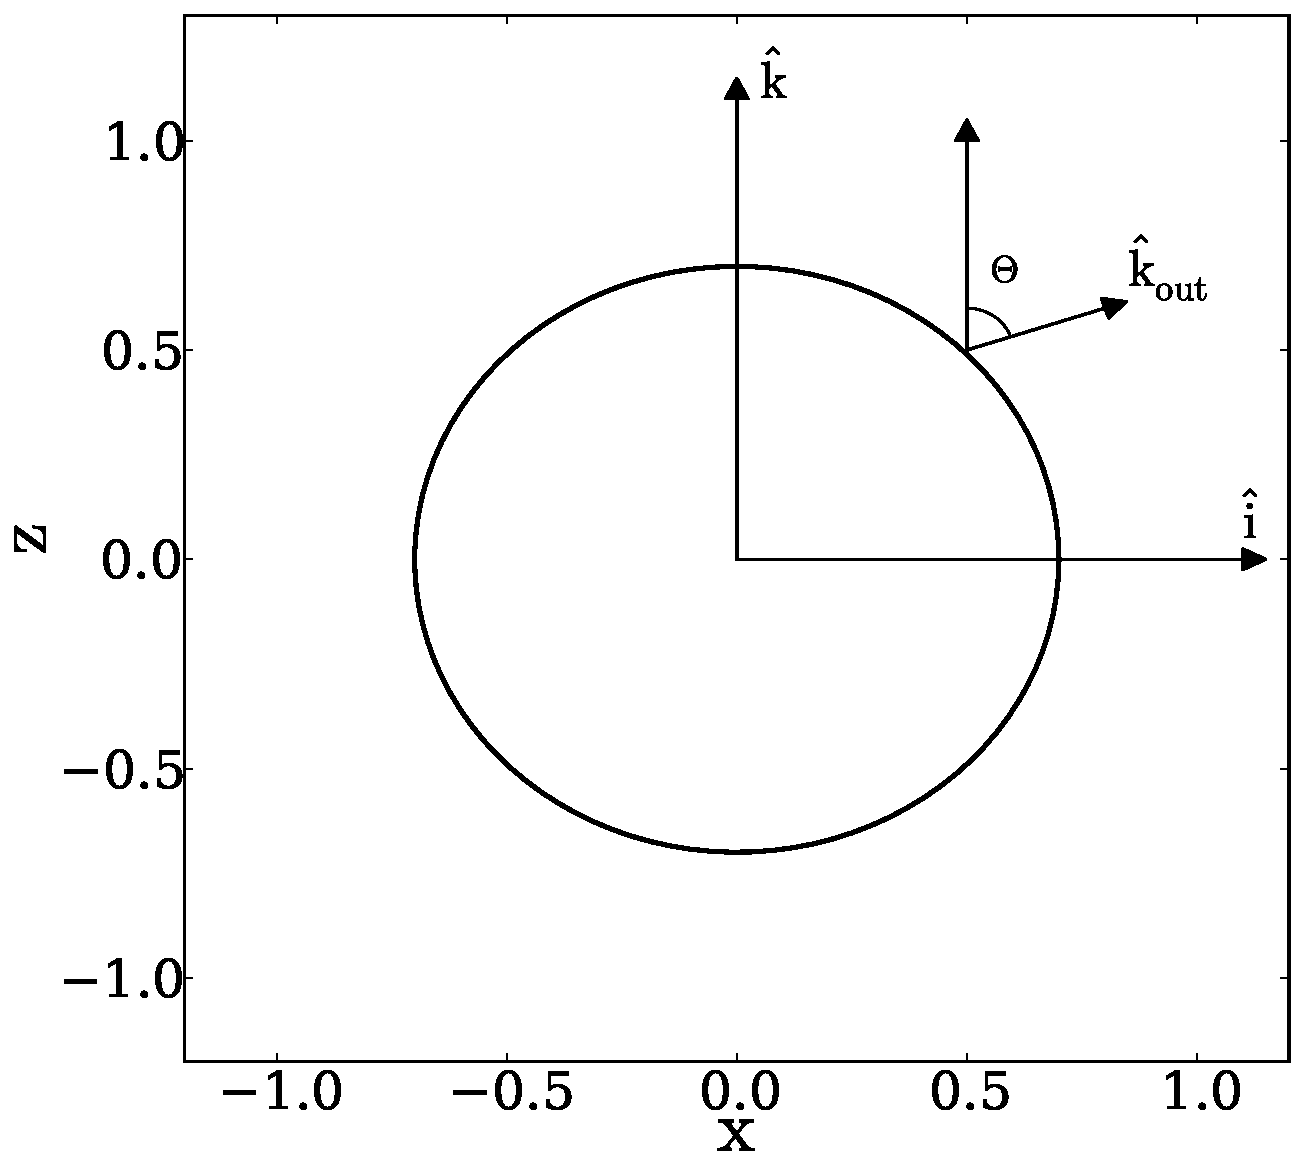
\includegraphics[width=0.4\textwidth]{f1.pdf}
\end{center}
\caption{Geometry of the gas distribution. The angular velocity vector
  is parallel to the unit vector $\hat{k}$. In order to describe the
  departures from spherical symmetry we use the polar angle $\theta$
  formed by the direction of the outgoing photons with respecto to the
  $z$-axis. We define define the variable $\mu\equiv\cos\theta$ to
  report to present our results.
    \label{fig:geometry}}  
\end{figure}



\begin{figure*}
\begin{center}
  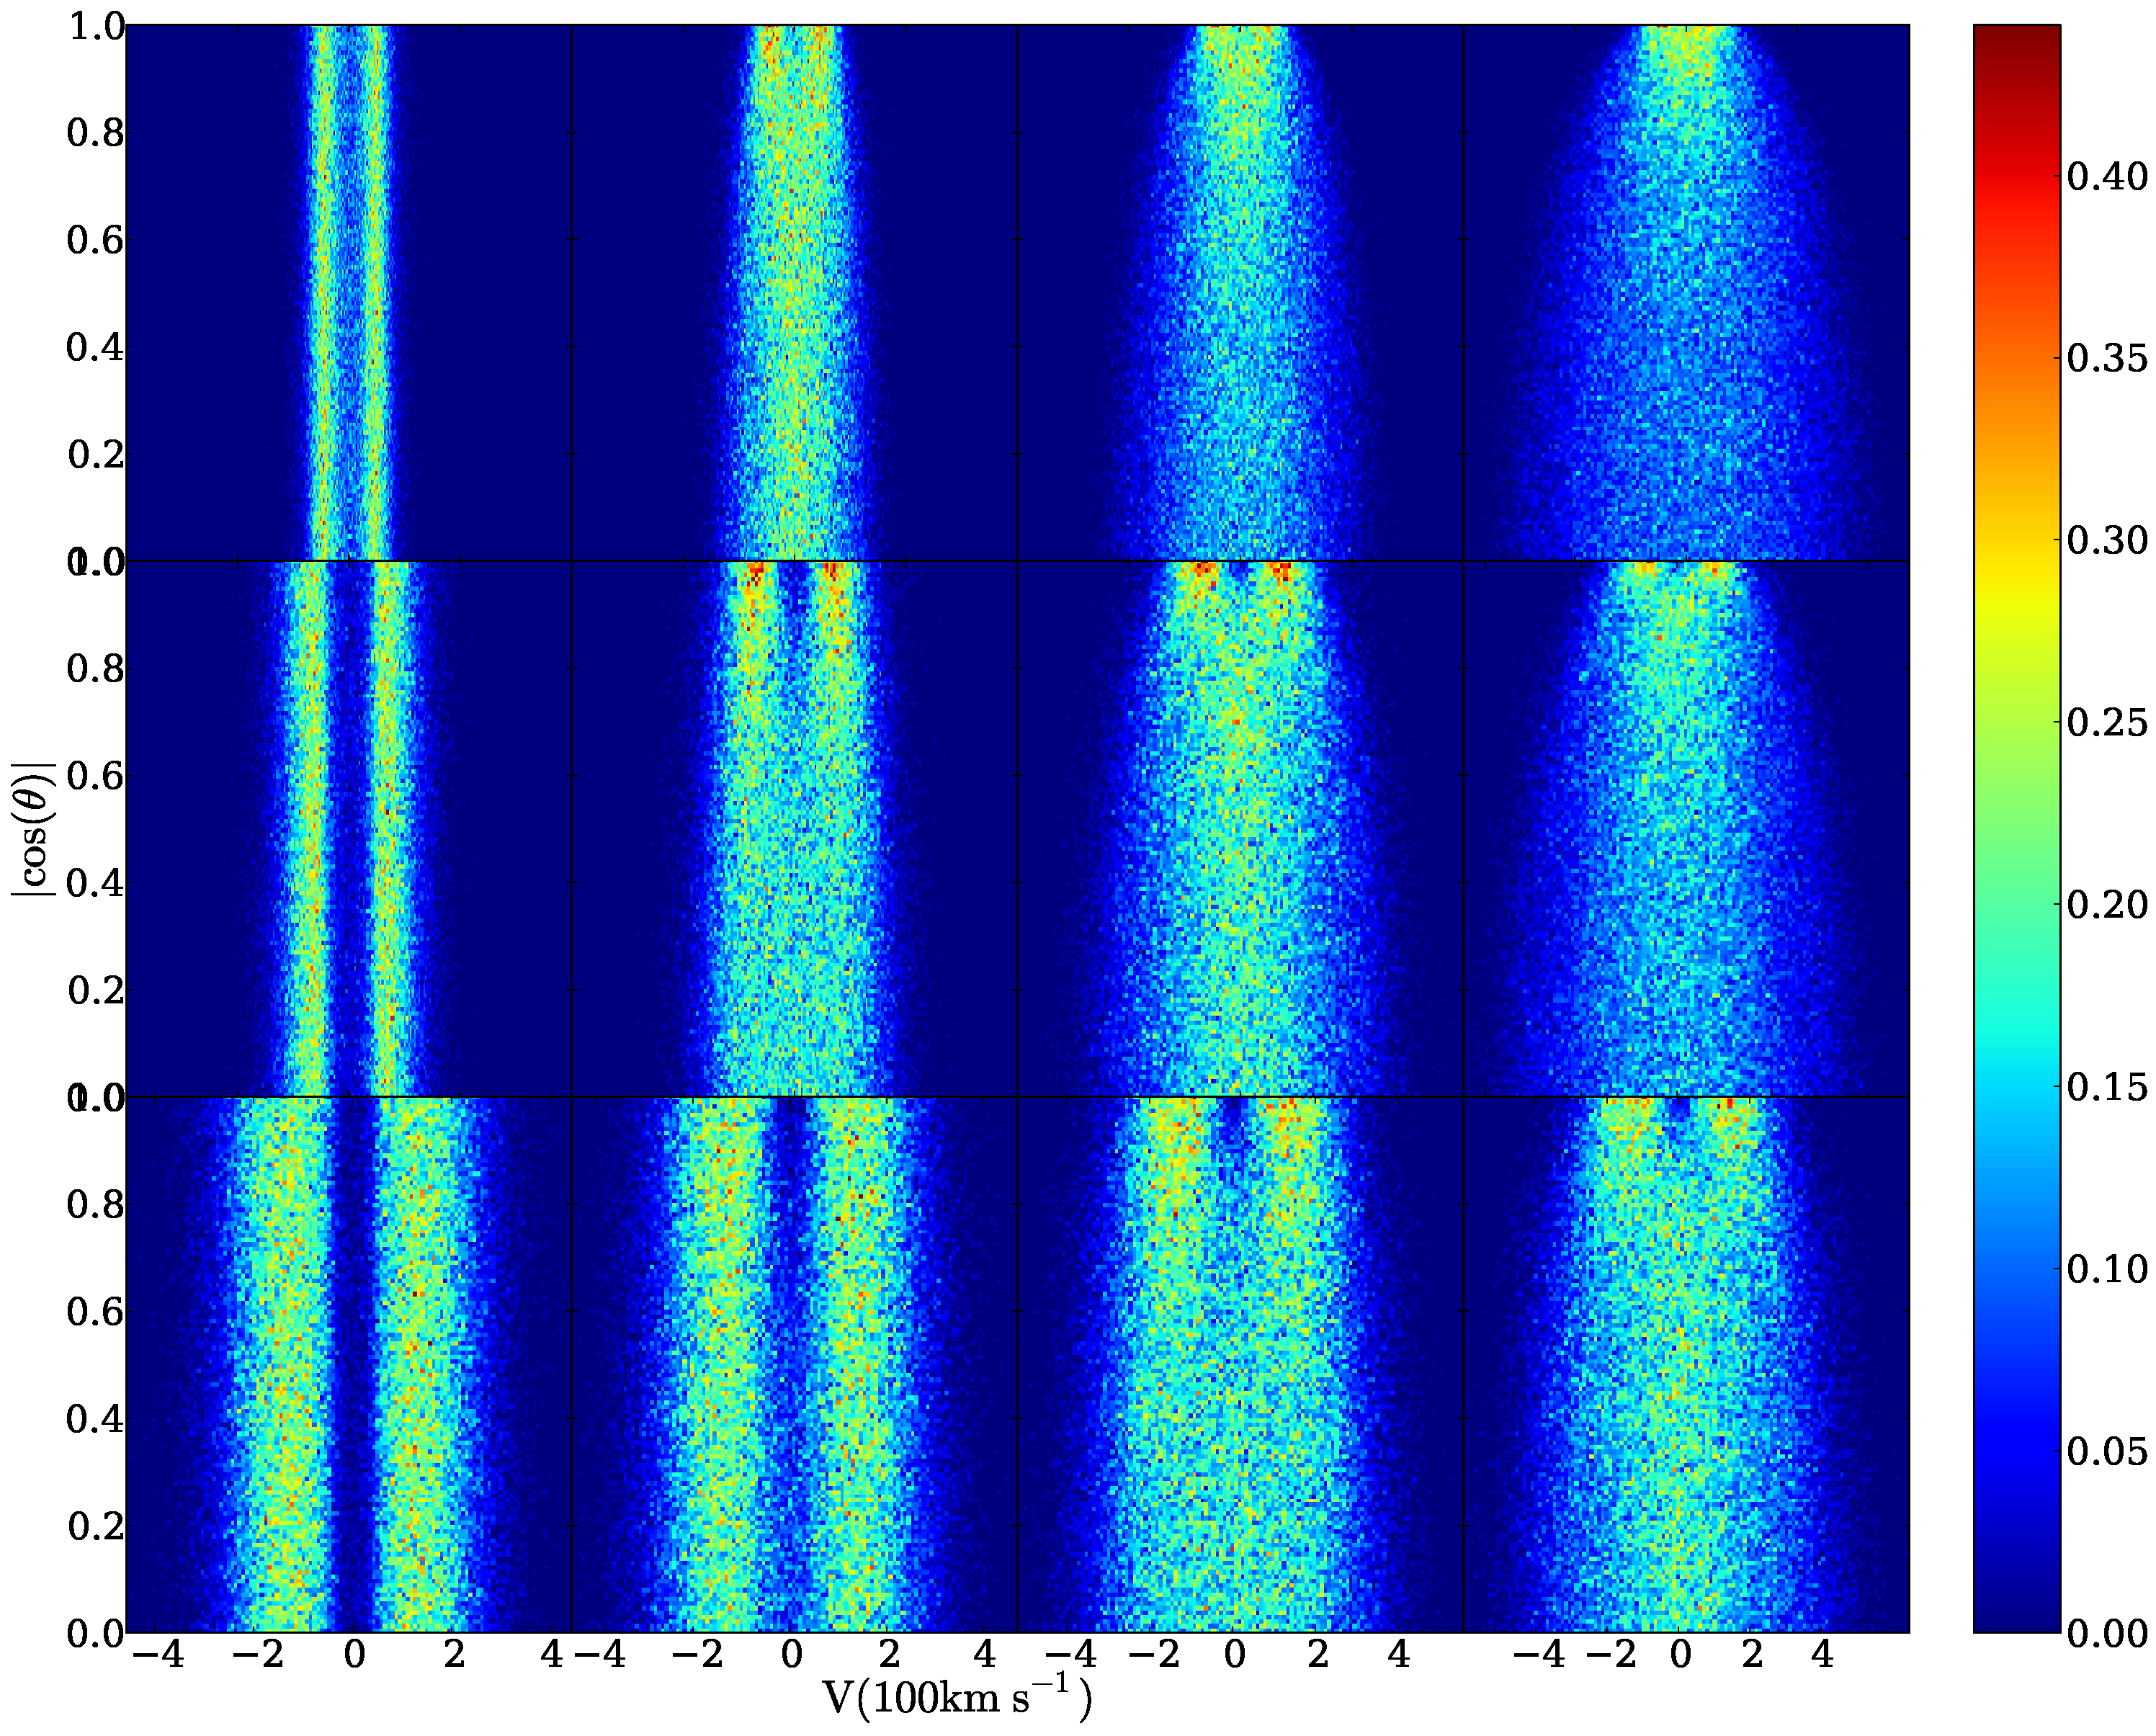
\includegraphics[width=0.95\textwidth]{f2.pdf}
\end{center}
\caption{
2D histogram showing the number of photons that escape with frecuency
$x$ forming an angle $\theta$ (parameterized as $\cos\theta$) with the
rotationa axis. The rotational velocity ($0,100,200,300$\kms)
increases from left to right and the optical depth ($10^5$, $10^6$,
$10^7$) from top to bottom. The \ly photons are initialized at the
center of the sphere.
\label{fig:CentralSpec} }   
\end{figure*}


\begin{figure*}
\begin{center}
  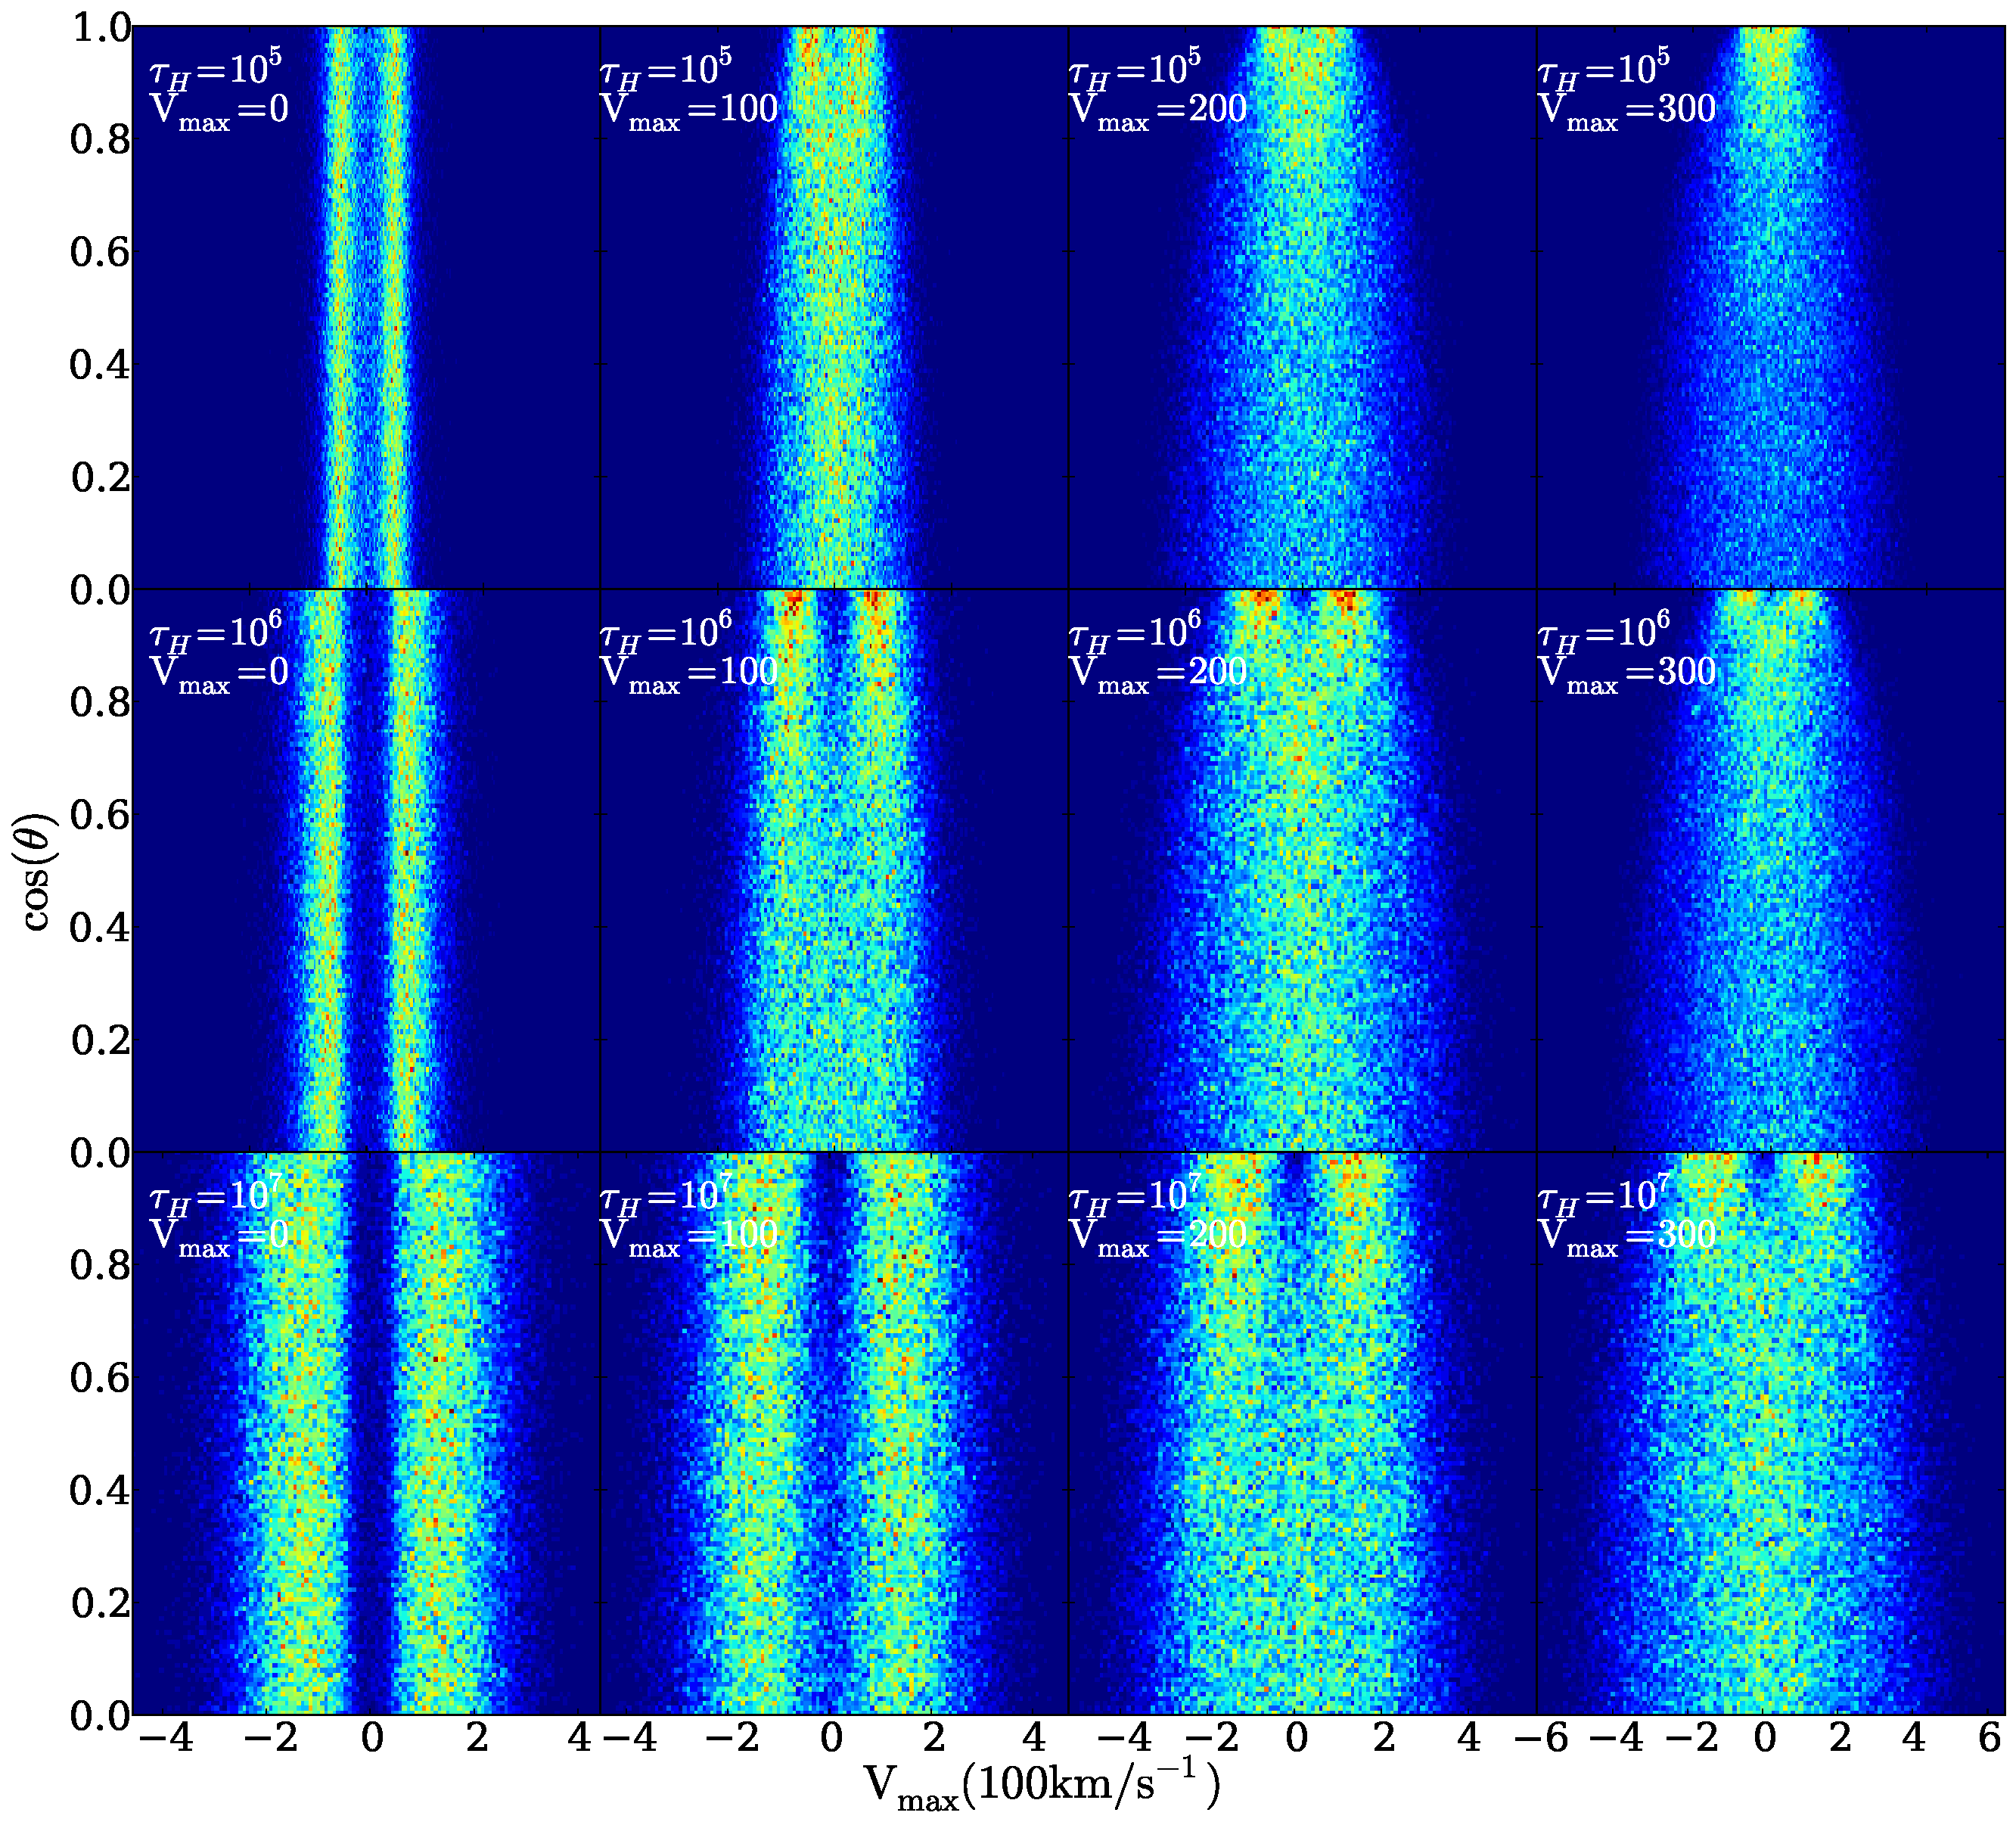
\includegraphics[width=0.95\textwidth]{f3.pdf}
\end{center}
\caption{Same as Figure \ref{fig:CentralSpec} for \ly photons
  initialized homogeneously throughout the sphere.
    \label{fig:HomSpec}}  
\end{figure*}

\begin{figure*}
\begin{center}
  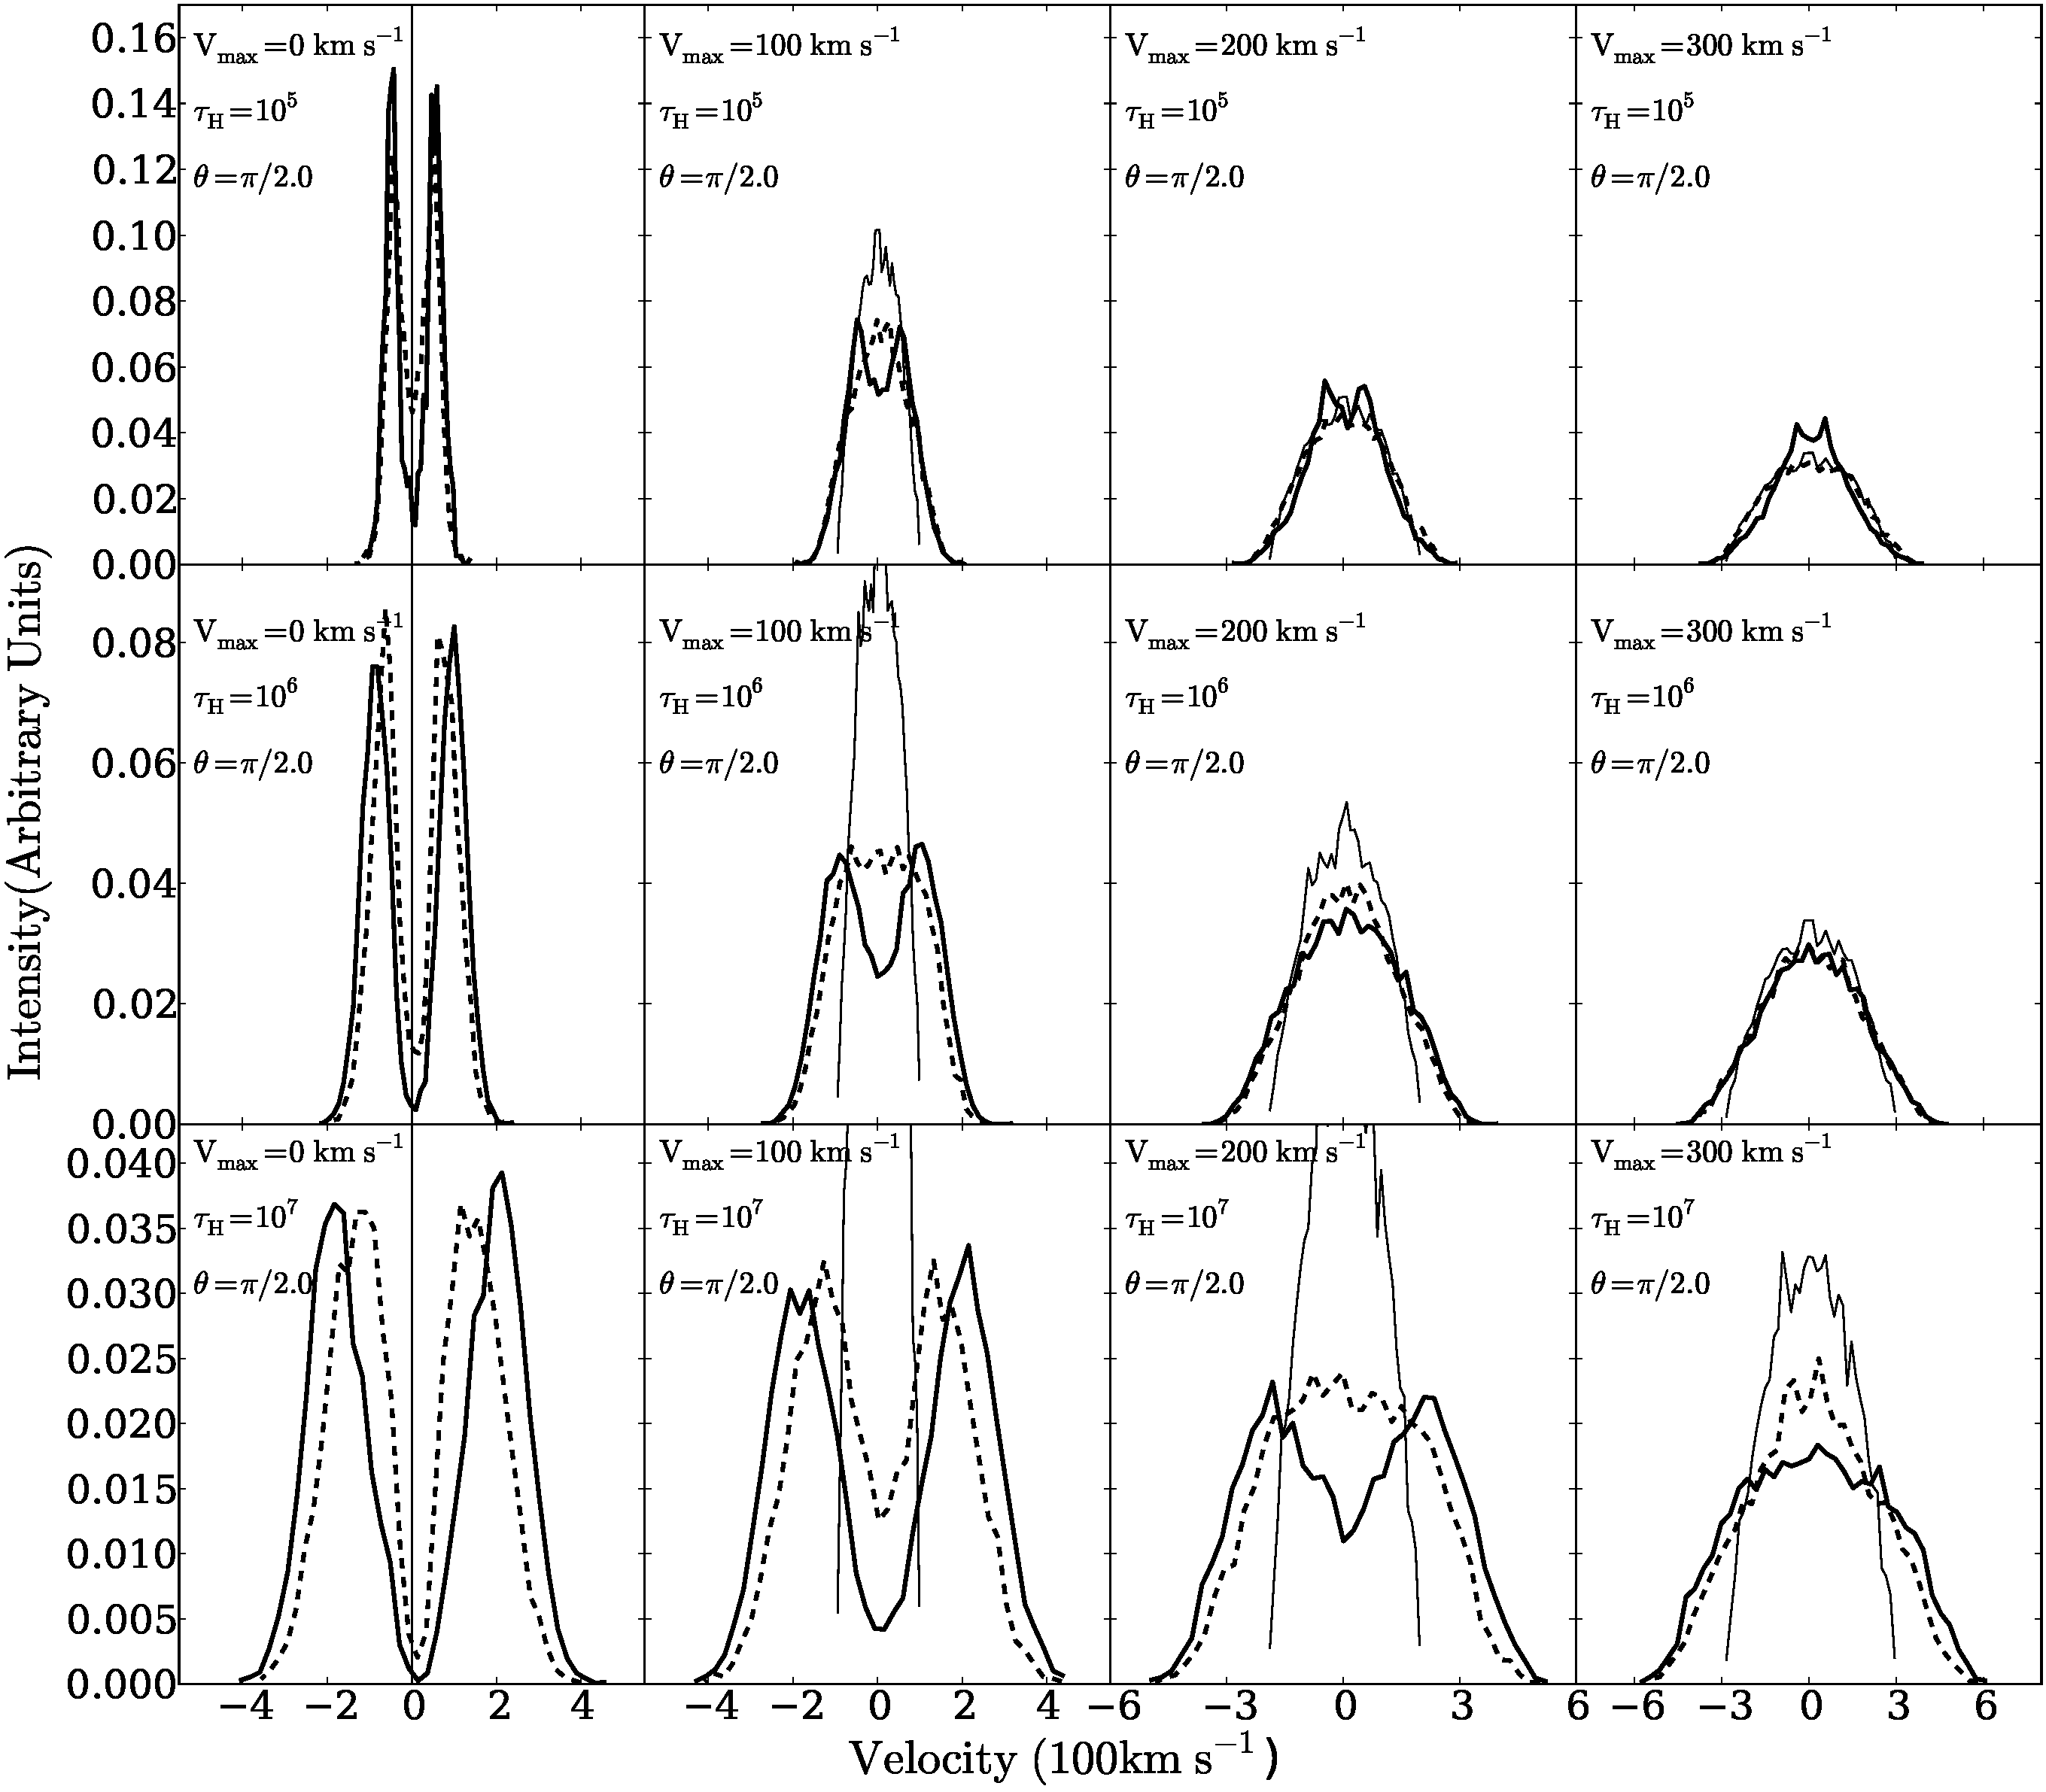
\includegraphics[width=0.95\textwidth]{f4.pdf}
\end{center}
\caption{Shape of the \ly line for different maximum rotational
  velocities for a viewing angle perpendicular to the rotation axis
  ($|\mu|\sim 0$). The continuous (dashed) line represents the central
  (homogeneous) source distributions.  The panels follow the same
  correspondence as Figures \ref{fig:CentralSpec} and \ref{fig:HomSpec}.
    \label{fig:differentvelocities}}  
\end{figure*}


\subsection{Brief Description of the Radiative Transfer Codes}

Here we briefly describe the relevant points for the two radiative
transfer codes we have used. For a detailed description we refer the
reader to the original papers \cite{CLARA,DijkstraKramer}.

The codes follow the individual scatterings of \ly photons as they
travel through a 3D distribution of neutral Hydrogen. At each
scattering the frequency of the photon (in the laboratory frame) and
its direction of propagation change. This change in frequency is due
to the peculiar velocities of the Hydrogen atom that absorbed and
re-emitted the photon. If dust is present, the photon can interact
either with a Hydrogen atom or dust grain. In the case of a dust
interaction the photon can be either absorbed or scattered, this
probability is encoded in the dust albedo, $A$, which we chose to be
$1/2$. In order to obtain accurate values for the escape fraction of
photons in the presence of dust, we do not use any accelerating
mechanism in the radiative transfer. Once the photons escape the gas
distribution we store their direction at their direction of
propagation and frequency at their last scattering.

The photons are thus emitted in some region of the gas distribution
and follow a random walk in space and frequency until they escape the
gas distribution or are absorbed by a dust grain. The initialization
process for the \ly photons has to specify its position, frequency and
direction of propagation. In our case we select the initial frequency
to be exactly the \ly rest-frame frequency ($x=0$) and the direction of
propagation to be random following an flat probability distribution
over the sphere. A different initization that uses a Gaussian with a
velocity with equal to the thermal velocity, $12.8$\kms in our case,
should not introduce noticeable change given that our rotational
velocities span the range $100$-$300$\kms and the lines have velocity
widths on the order of $100$-$500$\kms.

The gas is completely defined by its geometry (i.e. sphere or slab),
temperature $T$, Hydrogen optical depth $\tau_{\rm H}$, dust optical
depth $\tau_{\rm a}$ and the bulk velocity field $\vec{v}$. Our codes
treat the gas as homogeneous in density ($\tau_{\rm H}$, $\tau_{\rm
  a}$) and temperature.  


\subsection{Grid of Simulated Galaxies}
\label{sec:models}

In the Monte Carlo calculations we follow the propagation of $N_{\gamma}=10^5$
numerical photons through different spherical galaxies. For each galaxy
we vary at least one of the following parameters: the maximum
rotational velocity $V_{\rm max}$, the hydrogen optical depth $\tau_{H}$,
the dust optical depth $\tau_{a}$ and the initial distribution of photons
with respect to the gas. There are $60$ models initial combining all
variations of the input parameters. Table \ref{table:models}
summarizes the different parameters.

Additionally, we have used two independently developed Monte Carlo
codes \citep{CLARA,DijkstraKramer} to perform the calculations. The
results we report are robust in the sense that they are obtained by
both codes.  

\begin{table}
\begin{center}
\begin{tabular}{llc}\hline\hline
Physical Parameter (units) & Symbol & Values\\\hline
Velocity (\kms) & $V_{\rm max}$&$0,\ 50,\ 100,\ 200,\ 300$\\
Hydrogen Optical Depth & $\tau_{H} $ & $10^{5},\ 10^{6},\ 10^{7}$\\
Dust Optical Depth & $\tau_{a}$ & $0$,$1$\\
Photons Distributions & & Central, Homogeneous\\\hline\hline
\end{tabular}
\caption{
  Summary of Physical Parameters of our Monte Carlo Simulations.} 
\label{table:models}
\end{center}
\end{table}




\section{Results}
\label{sec:results}

The central results of this paper are summarized in Figures
\ref{fig:CentralSpec} and \ref{fig:HomSpec}. They show 2D histograms
of the escape frequency $x$ and outgoing angle $\theta$ parameterized by
$|\mu|$. Constructing the emission line with photons around a value
of $\mu$ would gives us the emission detected by an observer located at an
angle $\theta$ with respect to the rotation axis. We have veryfied
that the solutions are indeed symmetric with respect to $\mu=0$.  

From these Figures we can see that the line properties change with
rotational velocity and depend on the viewing angle $\theta$.  In the
next subsections we describe in  detail the changes of the morphology
with velocity, optical depth and viewing angle. We characterize the
line morphology by its total intensity, the full width at half maximum
(FWHM) and the location of the peak maxima. In order to interpret the
morphological changes in the line we also report the median number of
scatter for each \ly photon in the simulation. For the models where
dust is included we measure the escape fraction as a function of
rotational velocity.  

\subsection{Line Morphology}
\label{sec:angles}

The first column in both Figures \ref{fig:CentralSpec} and
\ref{fig:HomSpec} shows that for the static sphere the line properties
are independent of $|\mu|$, as it is expected due
to the spherical symmetry. However, for increasing rotational
velocities, at a fixed optical depth, there are clear signs that this
symmetry is broken. 

If the viewing angle is aligned witht the rotation axis, $|\mu|\sim
1$, the \ly line keeps a double peak with some changes as a function
of the rotational velocity that are easier to spot in models where the
\ly photons are homogeneously distributen than in the case of central
emission. 

However, for a line of sight perpendicular to the rotation
axis, $|\mu|\sim 0$, the impact of rotation is larger.  This is clear
in  Figure \ref{fig:differentvelocities} where we present the
different line morphologies for $|\mu|\sim 0$ for both the homogeneous
and central configurations. The panels have the same distribution as
Figures \ref{fig:CentralSpec} and \ref{fig:HomSpec}.  

For this case of $|\mu|\sim 0$, there are three clear effects on the
line's morphology as the rotational velocity increases. First, the
line broadens; second, the double peaks reduce their intensity; and
third, the intensity at the line center rises. The last two effects
merge to give the impression that the double peaks are merged into one
at high rotational velocities, a result that is evident for the
homogeneously distributed sources as shown in the dashed lines of
Figure \ref{fig:differentvelocities}. 


\subsection{Integrated Line Intensity}

\begin{figure}
\begin{center}
  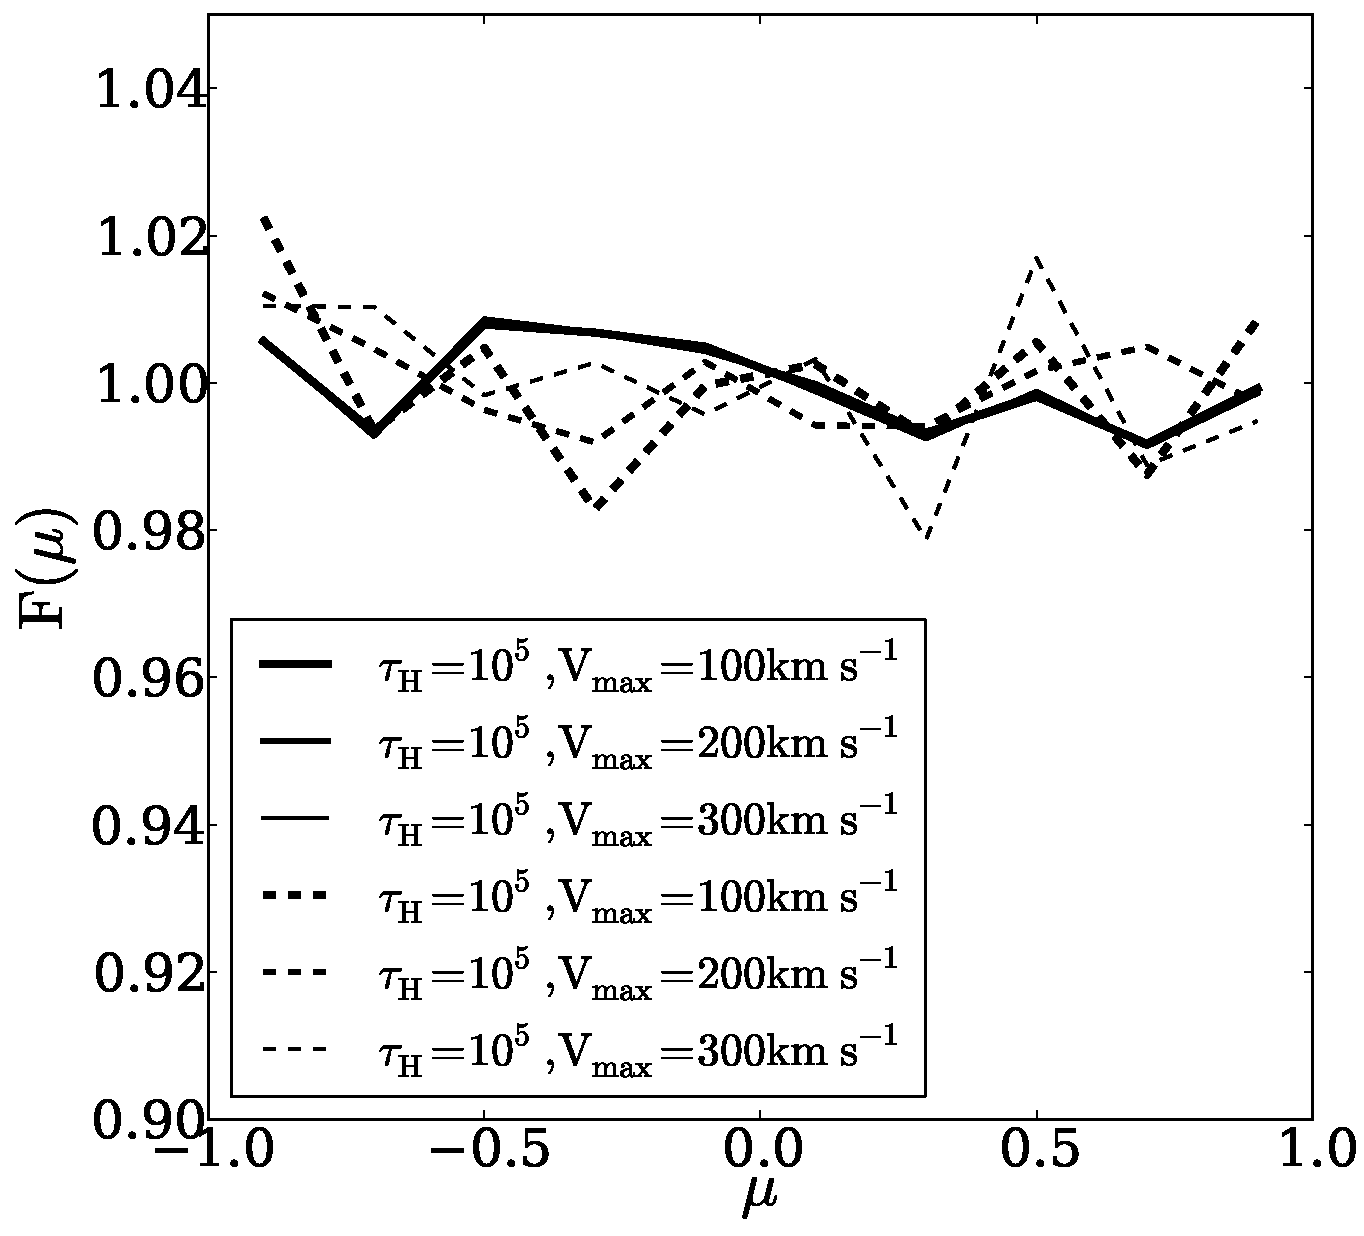
\includegraphics[width=0.4\textwidth]{f5.pdf}
\end{center}
\caption{Integrated flux distribution, $F(\mu)$, as a function of the
  viewing angle as parameterized by $\mu$. We show the results for the
  homogeneous source distribution in models with rotational velocities
  $0$\kms, $300$\kms and  optical depths $10^5$, $10^6$ and $10^7$. We
  see that the distribution is flat, meaning that the flux for all
  viewing angles is the same. The results for the central sources are
  similar. 
\label{fig:muhisto}}
\end{figure}

We consider possible variations in the integrated flux with respect to
$\theta$. We define the normalized flux seen by an observer at an
angle $\mu$ by: \begin{equation}
F(\mu) = \frac{2\Delta N}{N\Delta \mu}, 
\end{equation} 
%
where $\mu=\cos\Theta$, $N$ is the total number of outgoing photons,
$\Delta N$ is the number of photons in an angular bin $\Delta
\Theta$. This definition satisfies the condition
$\int_{-1}^{1}F(\mu)d\mu/2=1$. 

Figure \ref{fig:muhisto} shows a flat $F(\mu)$ for all models. It
means that in spite of the different morphologies, the integrated flux
is the same for all sight angles.  
	

\subsection{Full Width at Half Maximum}
\label{sec:widthpeak}


\begin{figure*}
\begin{center}
  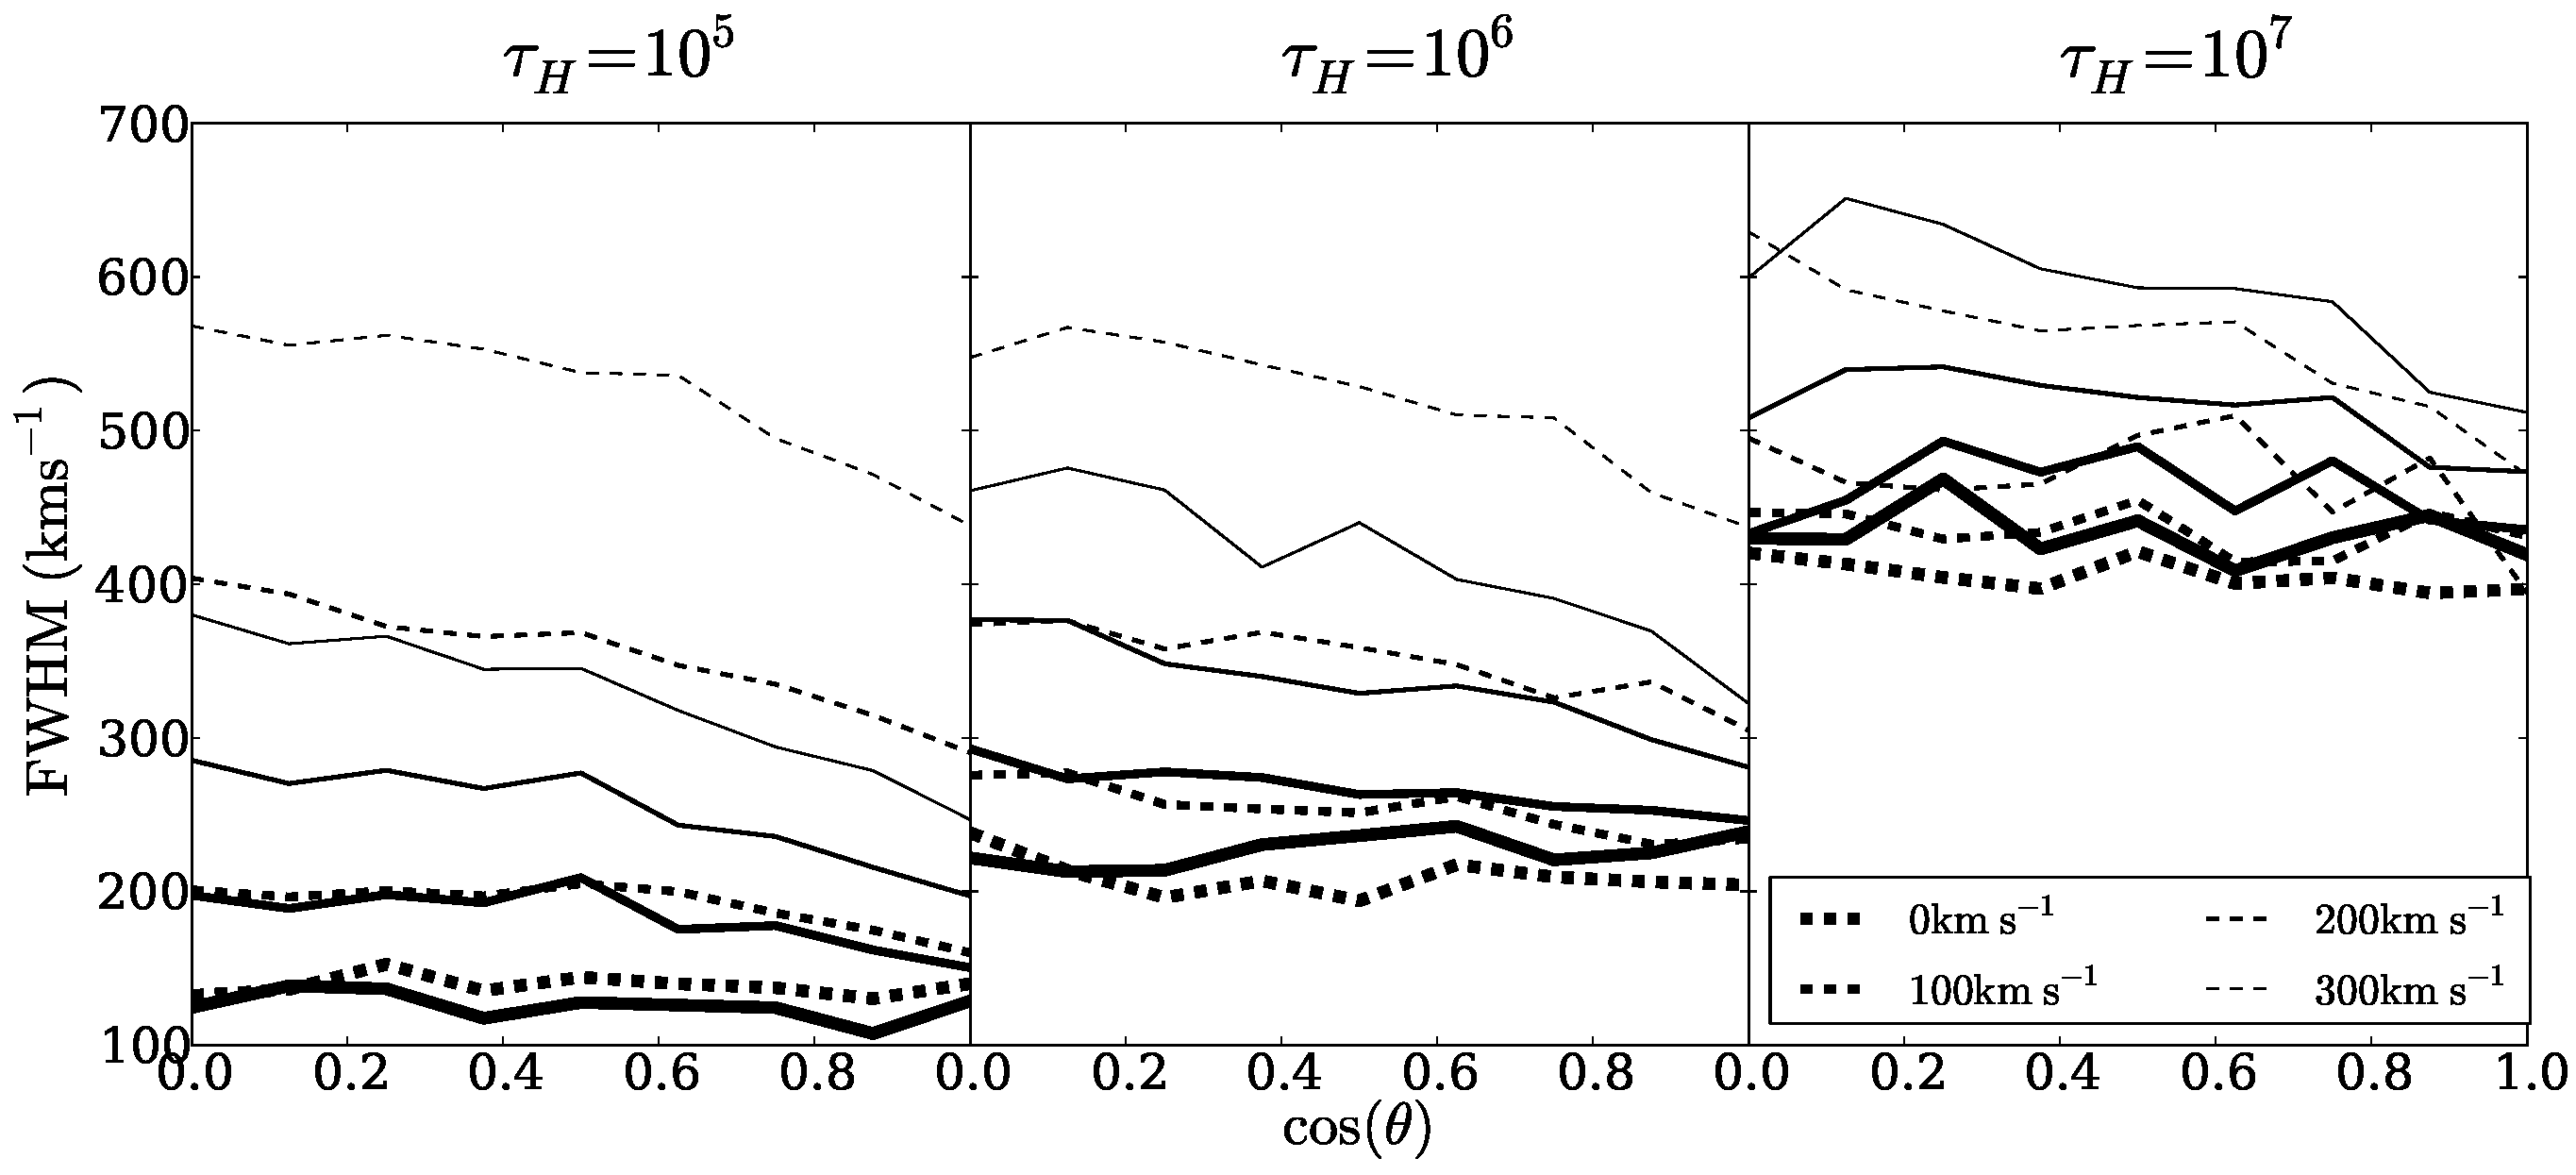
\includegraphics[width=0.95\textwidth]{f6.pdf}
\end{center}
  \caption{FWHM for the non-dusty models as a function of the viewing
  angle parameterized by $\mu\equiv\cos\theta$. 
  Continuous (dashed) lines  correspond to central (homogeneous)
  source distributions. The general trend is of an decreasing FWHM as
  the line of sight becomes parallel to the rotation axis. 
  \label{fig:widthvsmu}} 
\end{figure*}

\begin{figure*}
\begin{center}
  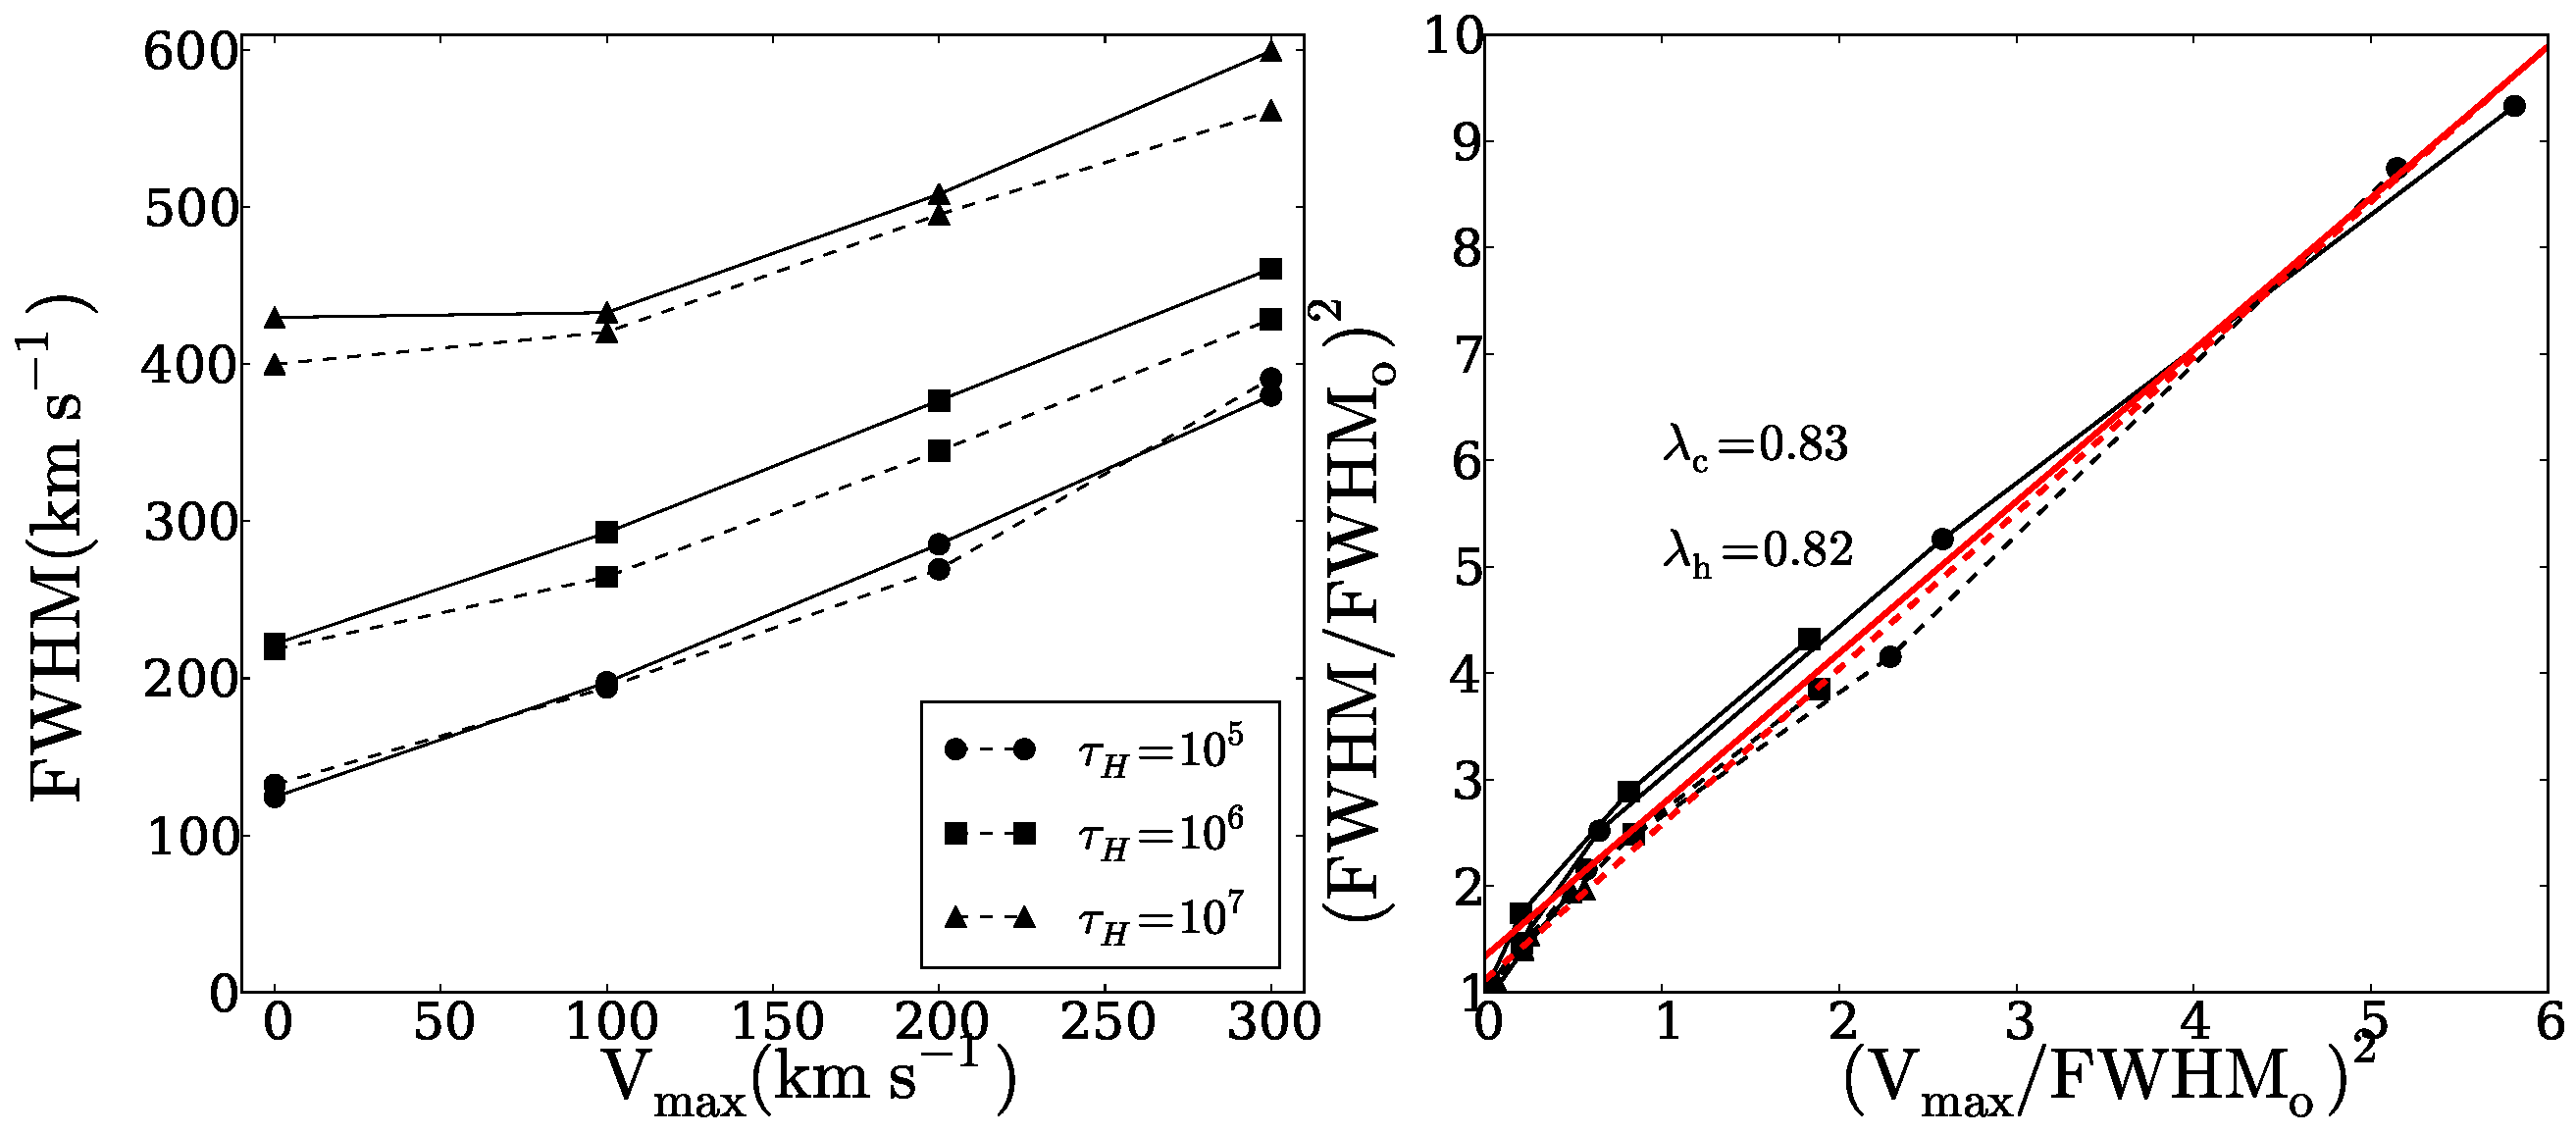
\includegraphics[width=0.95\textwidth]{f7.pdf}
\end{center}
\caption{FWHM for the non-dusty models as a function of
  rotational velocity $V_{\rm max}$. The left panel shows the
  results in velocity units while the right panel normalizes
  the data by the FWHM in the static case. 
  Continuous (dashed) lines  correspond to central (homogeneous)
  source distributions. The straight lines represent the fit to
  the data using the expression in Eq. (\ref{eq:fwhm}).
  \label{fig:widthsvsvelocity}}
\end{figure*}


We use the full width at half maximum (FWHM) to quantify the line
broadening. We measure this width from the velocity histogram by
finding the values of the velocities at half maximum. We use lineal
interpolation between histogram points to get a more precise value for
this width.

Figure \ref{fig:widthvsmu} shows the FWHM for all models as a function
of the viewing angle. The FWHM increases for decreasing values of
$\mu$ increases and increasing values of $V_{\rm max}$. In Figure
\ref{fig:widthvsvelocity} we fix $|\mu|<0.1$ and show the FWHM as a
function of rotational velocity. For this case we parametrize the
dependency of the line width with  $V_{\rm max}$ as

\begin{equation}
 {\rm FWHM}^2 = {\rm FWHM}_{0}^2 + V_{\rm max}^2/\lambda^2,
\label{eq:fwhm}
\end{equation}
%
where FWHM$_{0}$ is the velocity width in the static case and $\lambda$ 
is a positive scalar to be determined as a fit to the data. 

With this test we want to know to what extent the new velocity width
can be expressed as a quadratic sum of the two relevant velocities in
the problem. We fit simultaneously all the points corresponding to
central and homogeneous models to find $\lambda_{\rm c} = 0.84 \pm
0.06$ and $\lambda_{\rm h}= 0.54\pm 0.1$ respectively. 


\subsection{Line Maxima}
\label{sec:maxima}

\begin{figure*}
\begin{center}
  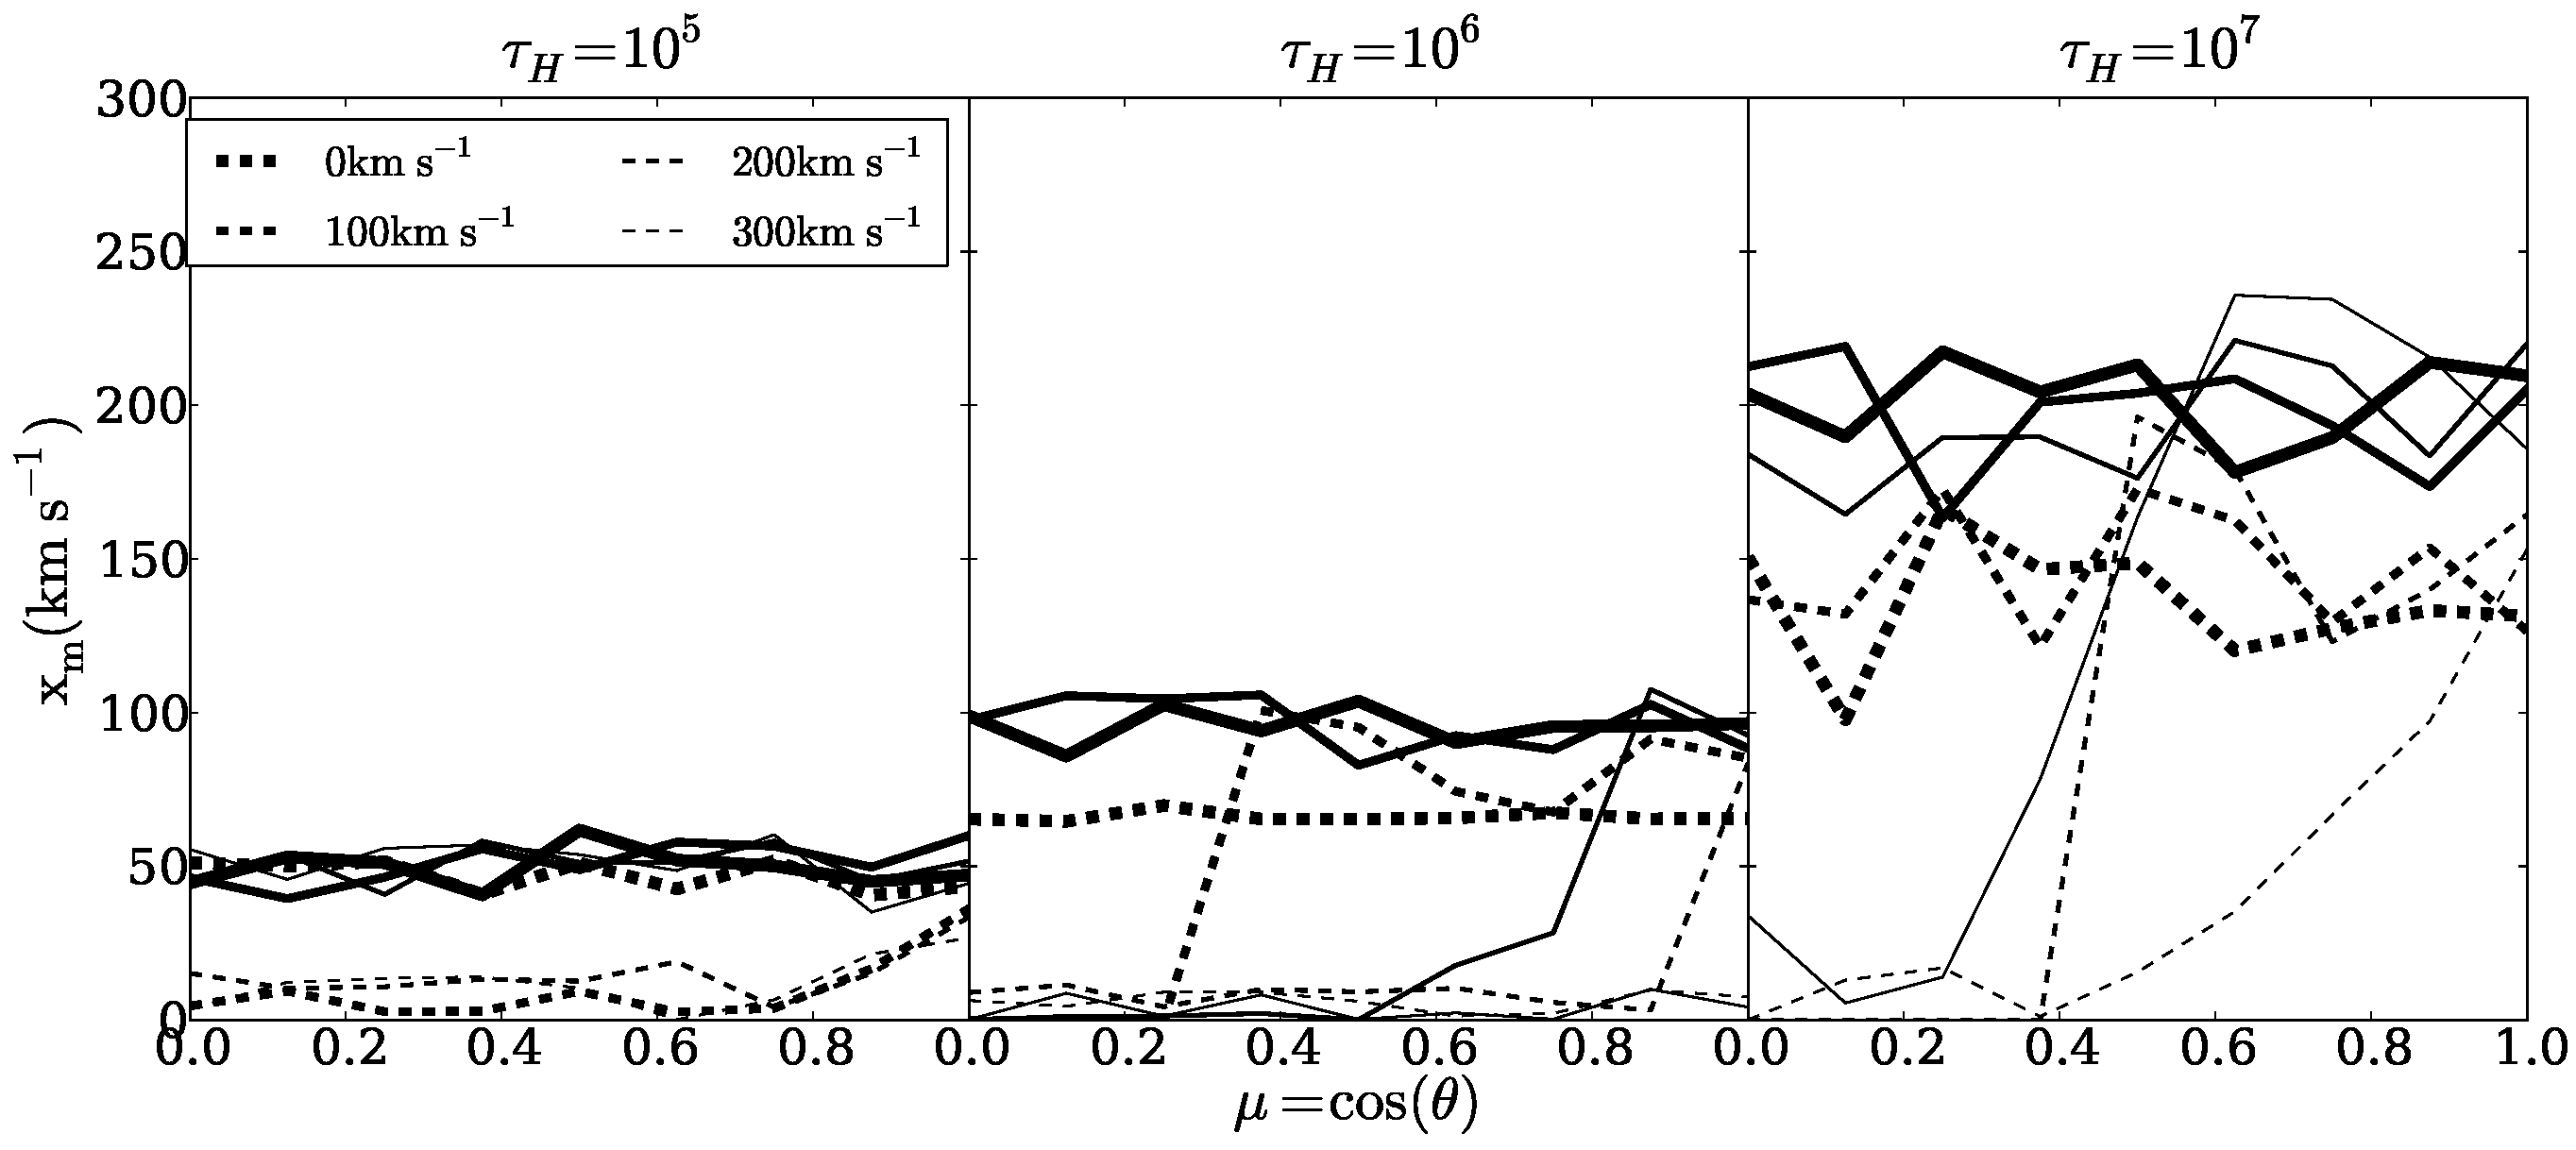
\includegraphics[width=0.95\textwidth]{f8.pdf}
\end{center}
\caption{Position of the line maxima as a function of maximum
  rotational   velocity $V_{\rm max}$. Continuous (dashed) lines
  correspond to   central (homogeneous) source distributions. A value
  of $x_{\rm     max}=0$ indicates that line becomes single
  peaked. \label{fig:maximumsvsvelocity}}
\end{figure*}

We measure the peak maxima position to quantify the transition from
double into single peak. We do this as a function of the viewing angle
$\theta$ and the maximum rotational velocity. The results are
summarized in Figure  \ref{fig:maximumsvsvelocity}. There are two
interesting features that deserve attention. First, for a viewing angle
parallel to the rotational axis ($\mu\sim 1.0$) the maxima of all
models are similar regardless of the rotational velocity. Second, at a
viewing angle perpendicular to the rotation axis ($\mu\sim 0.0$) there
is a good fraction of models that become single peaked, a feature that
appears more frequently for homogeneously distributed sources when all
the other parameters are equal.

\subsection{Dusty Clouds: Escape Fraction}
\label{sec:escapefraction}

\begin{table}
\begin{center}
\begin{tabular}{c ccc ccc}
\hline \hline
Source & $\tau_{H}$ & & & $\ V_{\rm max}$& & \\
Distribution& &  &  & (\kms) & & \\ 
& & 0 & 50 & 100 &200 & 300\\ \hline 
Homogeneous & $10^{5}$& 0.263 & 0.266 &  0.309 &  0.357 &  0.370  \\
            & $10^{6}$ & 0.289 &  0.289 &   0.309 &  0.360 &  0.393 \\
            &$10^{7}$ &  0.227 &  0.229 &  0.231 &  0.254 &  0.281 \\
Central & $10^{5}$ &  0.096 & 0.097 & 0.096 &  0.096 & 0.096 \\
  		&$10^{6}$ & 0.066 & 0.066 &  0.066 &  0.066 &  0.066 \\
 		&$10^{7}$ & 0.015 &  0.016 & 0.016 & 0.016 & 0.015 \\
\hline
\end{tabular}
\caption{
 Escape fraction values for all dusty models. } 
\label{table:escape}
\end{center}
\end{table}

\begin{figure*}
\begin{center}
  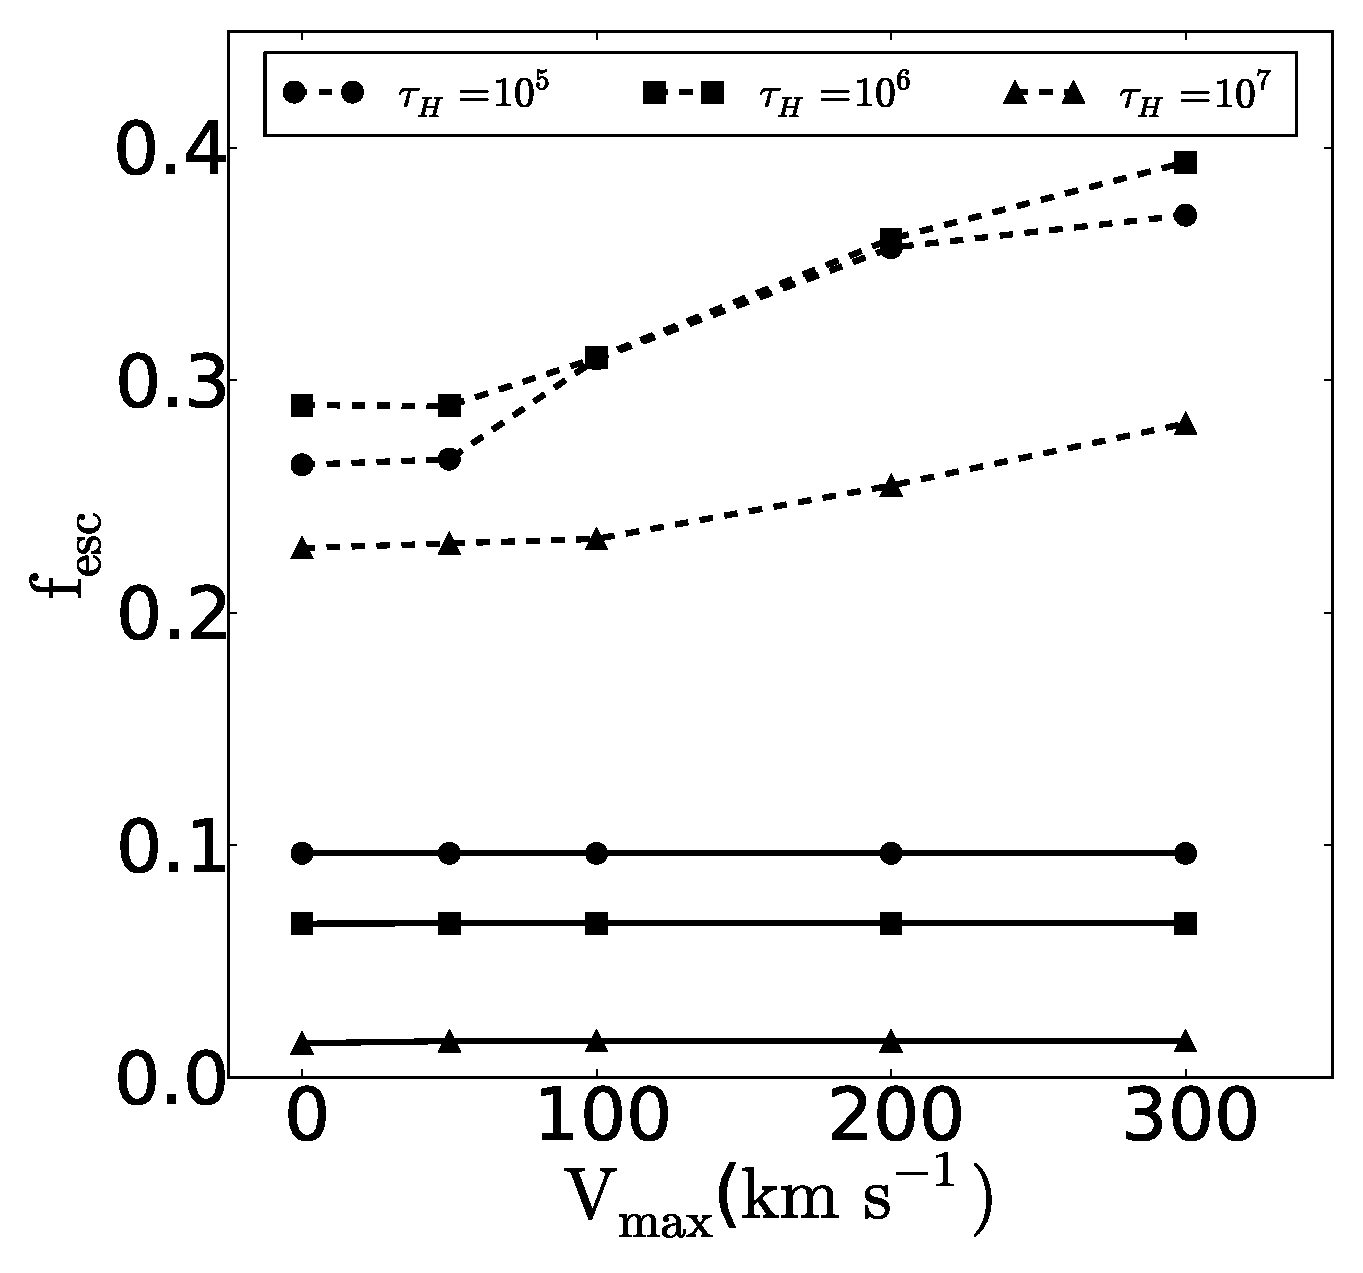
\includegraphics[width=0.40\textwidth]{f6.eps}
  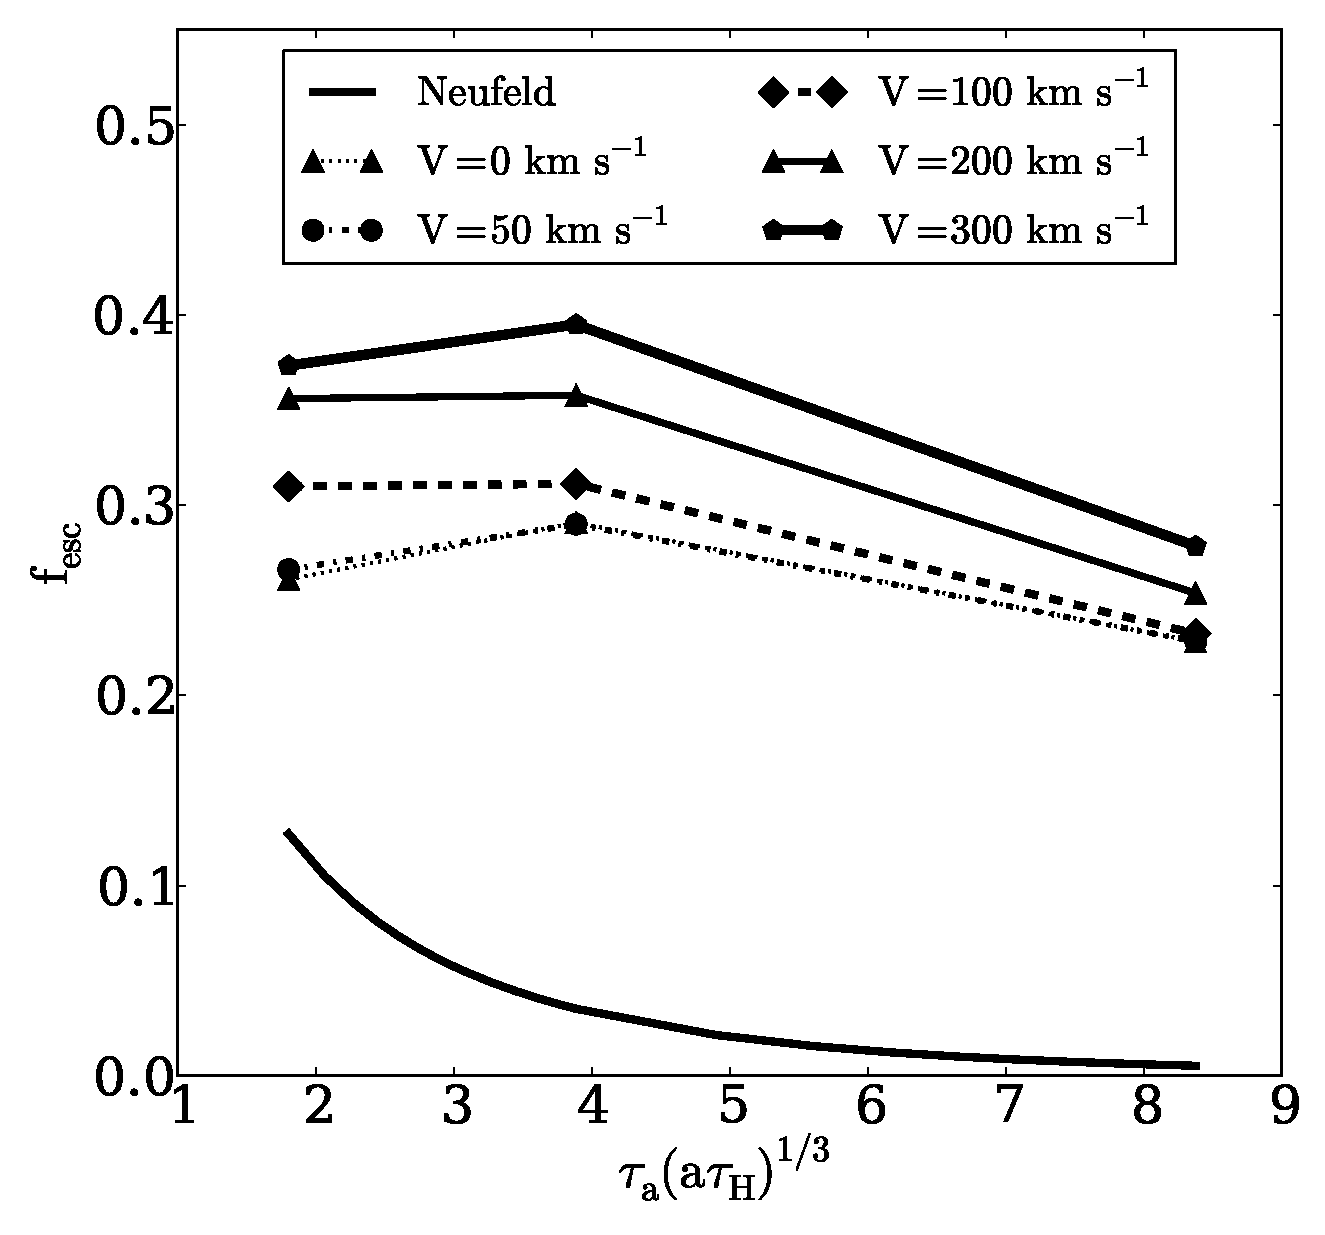
\includegraphics[width=0.40\textwidth]{f7.eps}
\end{center}
  \caption{Effects of rotation on the escape fraction. Left
    panel, escape fraction as a function of rotational velocity. All
    these models have $\tau_{a}=1$. The continuous (dashed) lines
    correspond to central (homogeneous) models. Right panel, escape
    fraction as a    function of the product $(a\tau_{\rm
      H})^{1/3}\tau_{A}$. The    analytic solution for the infinite
    slab is shown as a continuous    line. Different lines correspond
    to different rotational velocities for the homogeneous models.     
    \label{fig:escape_fraction}} 
\end{figure*}

We now estimate the escape fraction $f_{\rm esc}$ for the dusty models. Our main
result is that we do not find any dependence with the viewing angle
but there is a strong dependence with the rotational velocity for the
homogeneous models.

The left panel in Figure \ref{fig:escape_fraction} summarizes our
results. The left panel shows the escape fraction as a function of the
rotational velocity. To construct this Figure we take into account all
the photons regardless of its outgoing direction. We observe that the
curves for the central source distribution stay flat, while for the
homogeneous case there is a clear rise with rotational velocity.
Rotation has a higher relative impact in the models with low optical
depth. For instance, in models with $\tau_{\rm H}=10^5$, the static
escape fraction is $0.26$ and increases to $0.37$ for $V_{\rm
  max}=300$ \kms. Table \ref{table:escape} lists all the values for
the escape fraction.   

In the right panel of Figure \ref{fig:escape_fraction} we put these
results in the context of the analytic solution for the infinite slab
\citep{Neufeld90}. In Neufeld's set-up the analytic solution depends
uniquely on the product $(a\tau_{\rm   H})^{1/3}\tau_{A}$ where
$\tau_{A} = (1 - A)\tau_{a}$, valid only in the limit $a\tau_{\rm
  H}\gg 1$. The dashed lines in  the right panel of Figure
\ref{fig:escape_fraction} show the results for the different
rotational velocities for the homogeneous models. First of all we note
that the escape fraction does not increase significantly from
$\tau_{\rm H}=10^{5}$ to $\tau_{\rm H}=10^{6}$. This
counter-intuitive result is a consequence of the transition into the
'extremely' opaque regime,  which occurs roughly when $a\tau_{\rm{H}}
> 10^{3}$  e.g. \citep{Neufeld90}. 


\subsection{Average Number of Scatterings}
\label{sec:scatterings}

\begin{figure*}
\begin{center}
    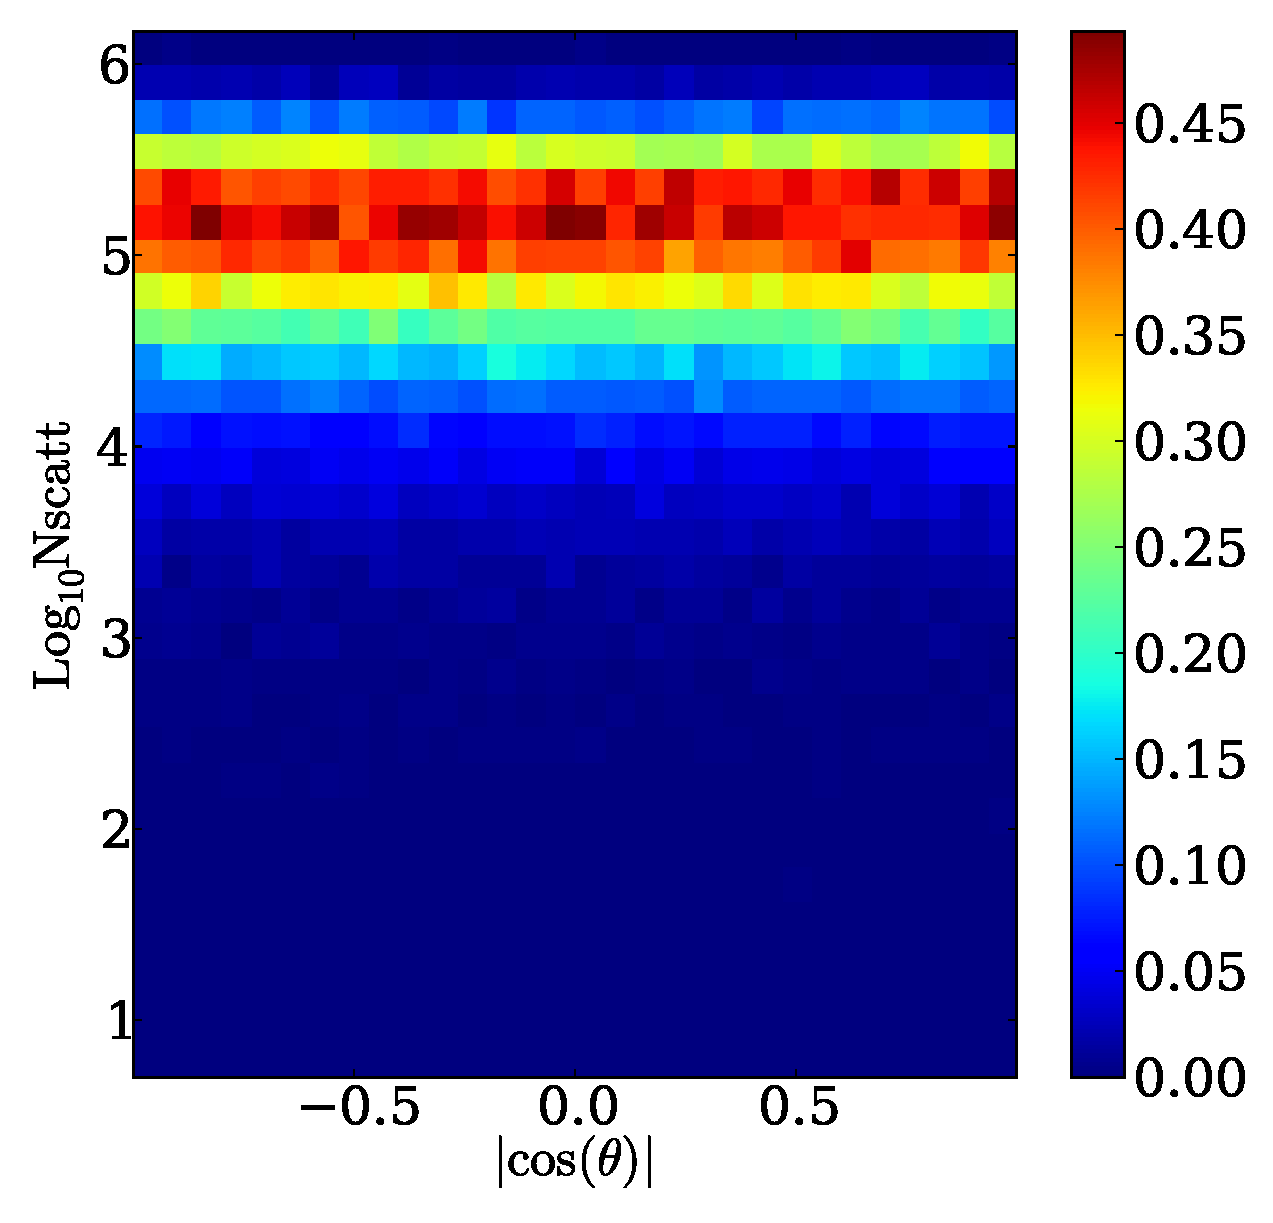
\includegraphics[width=0.45\textwidth]{nscattvsmu.eps}
    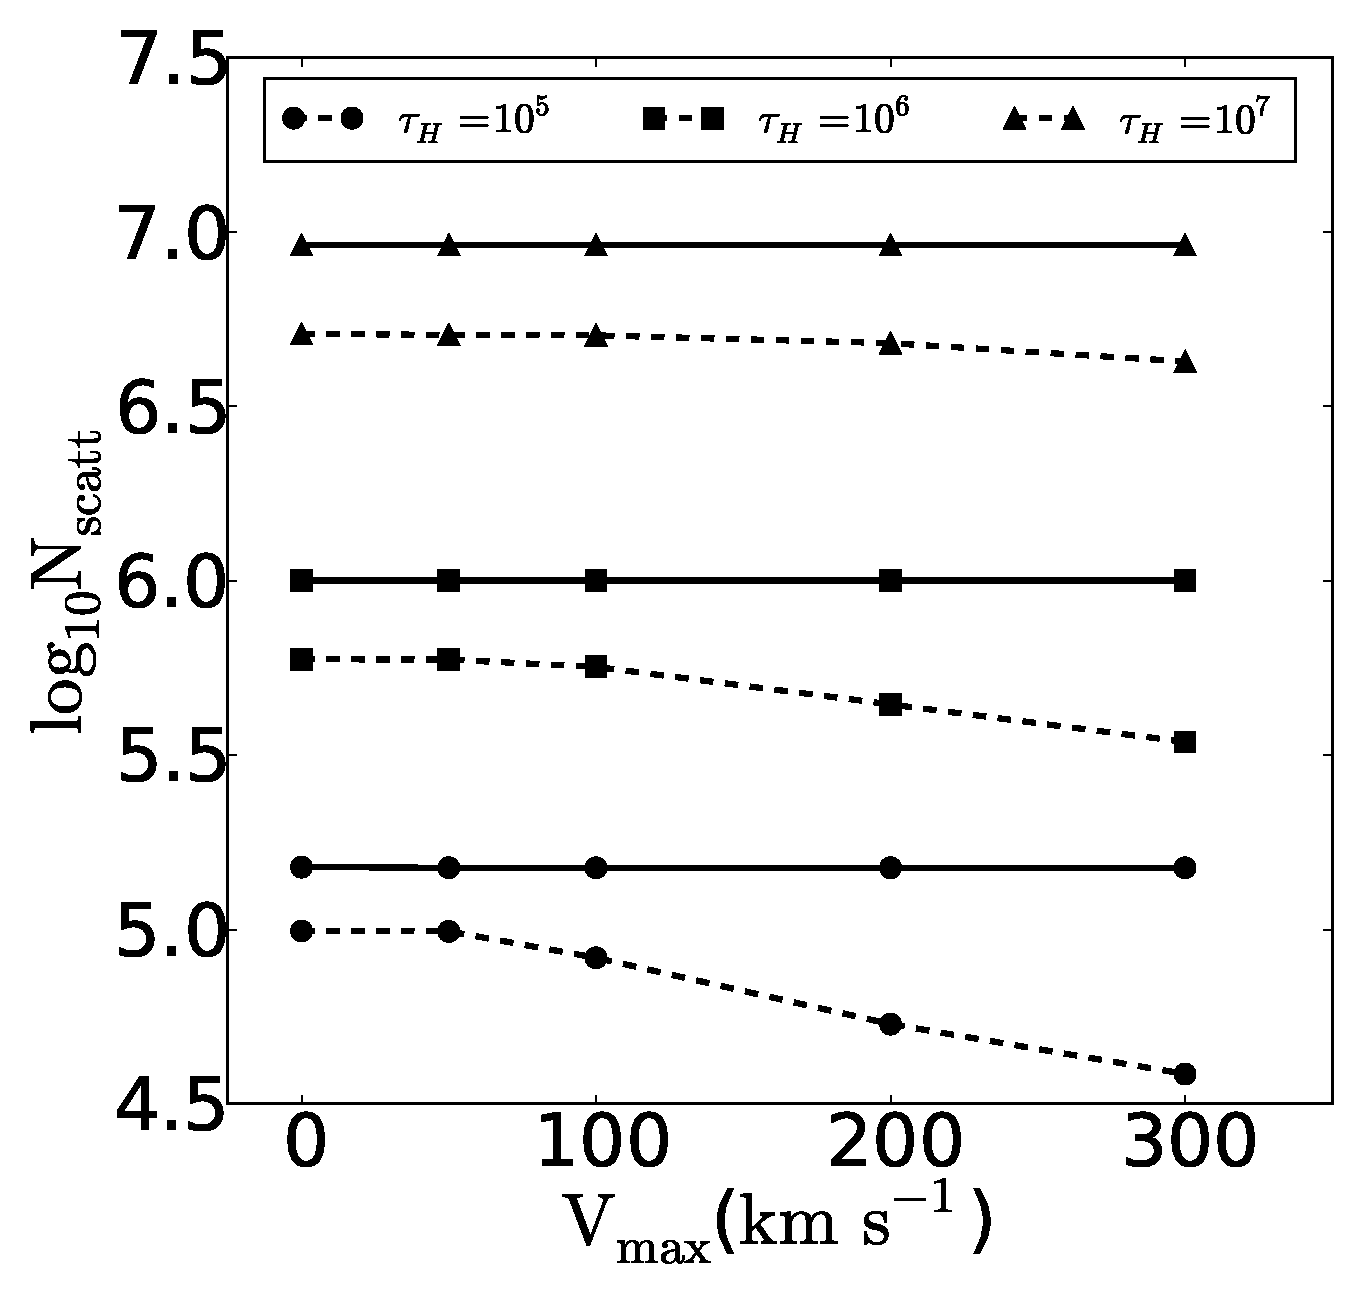
\includegraphics[width=0.45\textwidth]{f4.eps}
\end{center}
\caption{Logarithm of the average number of scatterings as function of
  $\mu$ (left panel) and the maximum rotational velocity $V_{\rm
    max}$. The left panel shows the behaviour for $\tau=10^{5}$ and
  $V_{max}=300$\kms but this independence of the independence between
  $N_{\rm scatt}$ and $\mu$ is kept for all models. 
  In the right panel the continuous (dashed) lines represent an
  central (homogeneous) distribution of sources; this shows the clear
  decrease in the number of scatterings for the homogenously
  distributed sources.
\label{fig:Nscatt} }    
\end{figure*}



\begin{figure*}
\begin{center}
  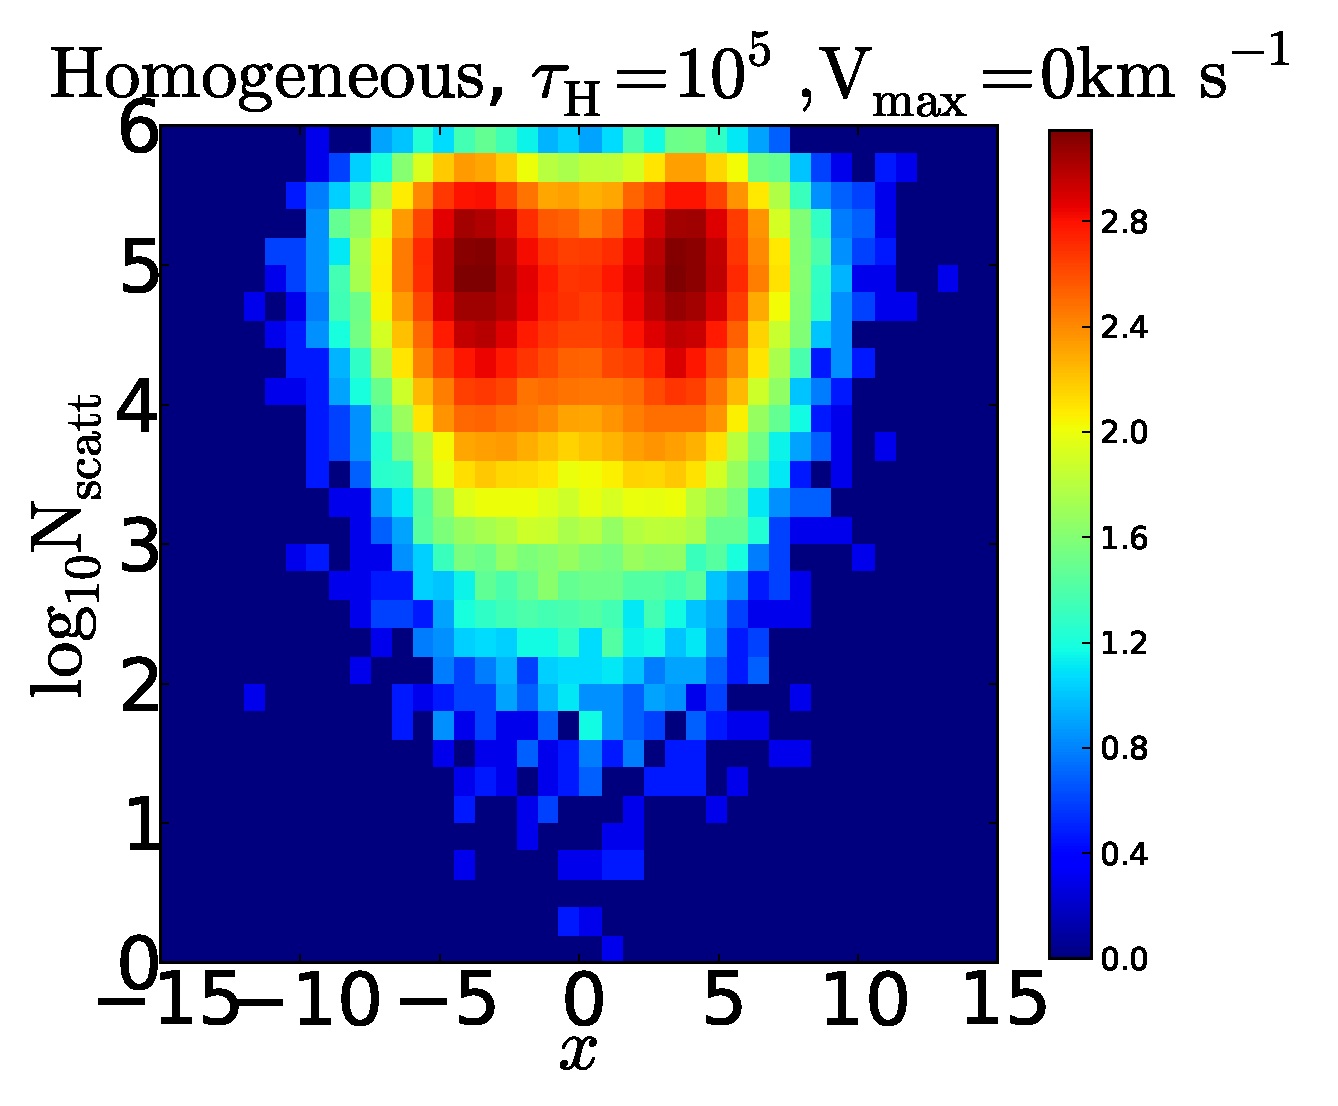
\includegraphics[width=0.48\textwidth]{f5_1.eps}
  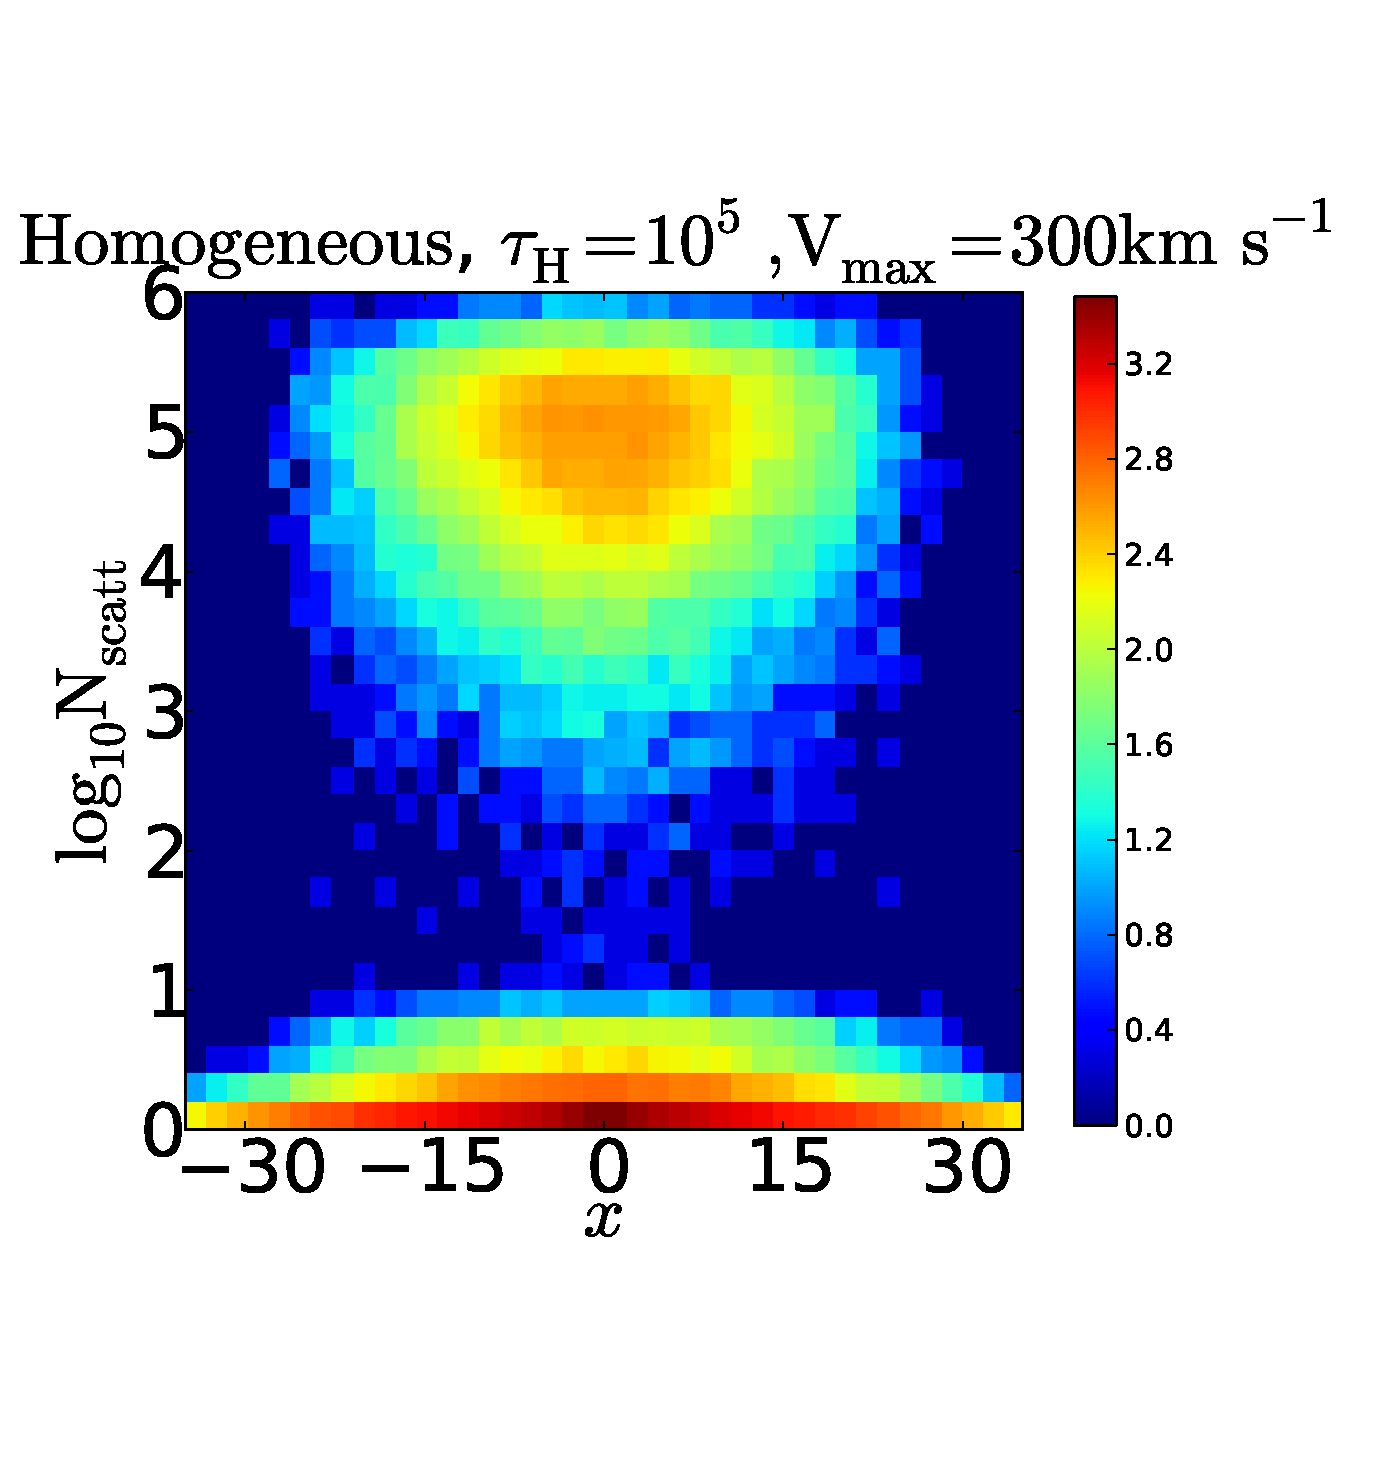
\includegraphics[width=0.48\textwidth]{f5_2.eps}
  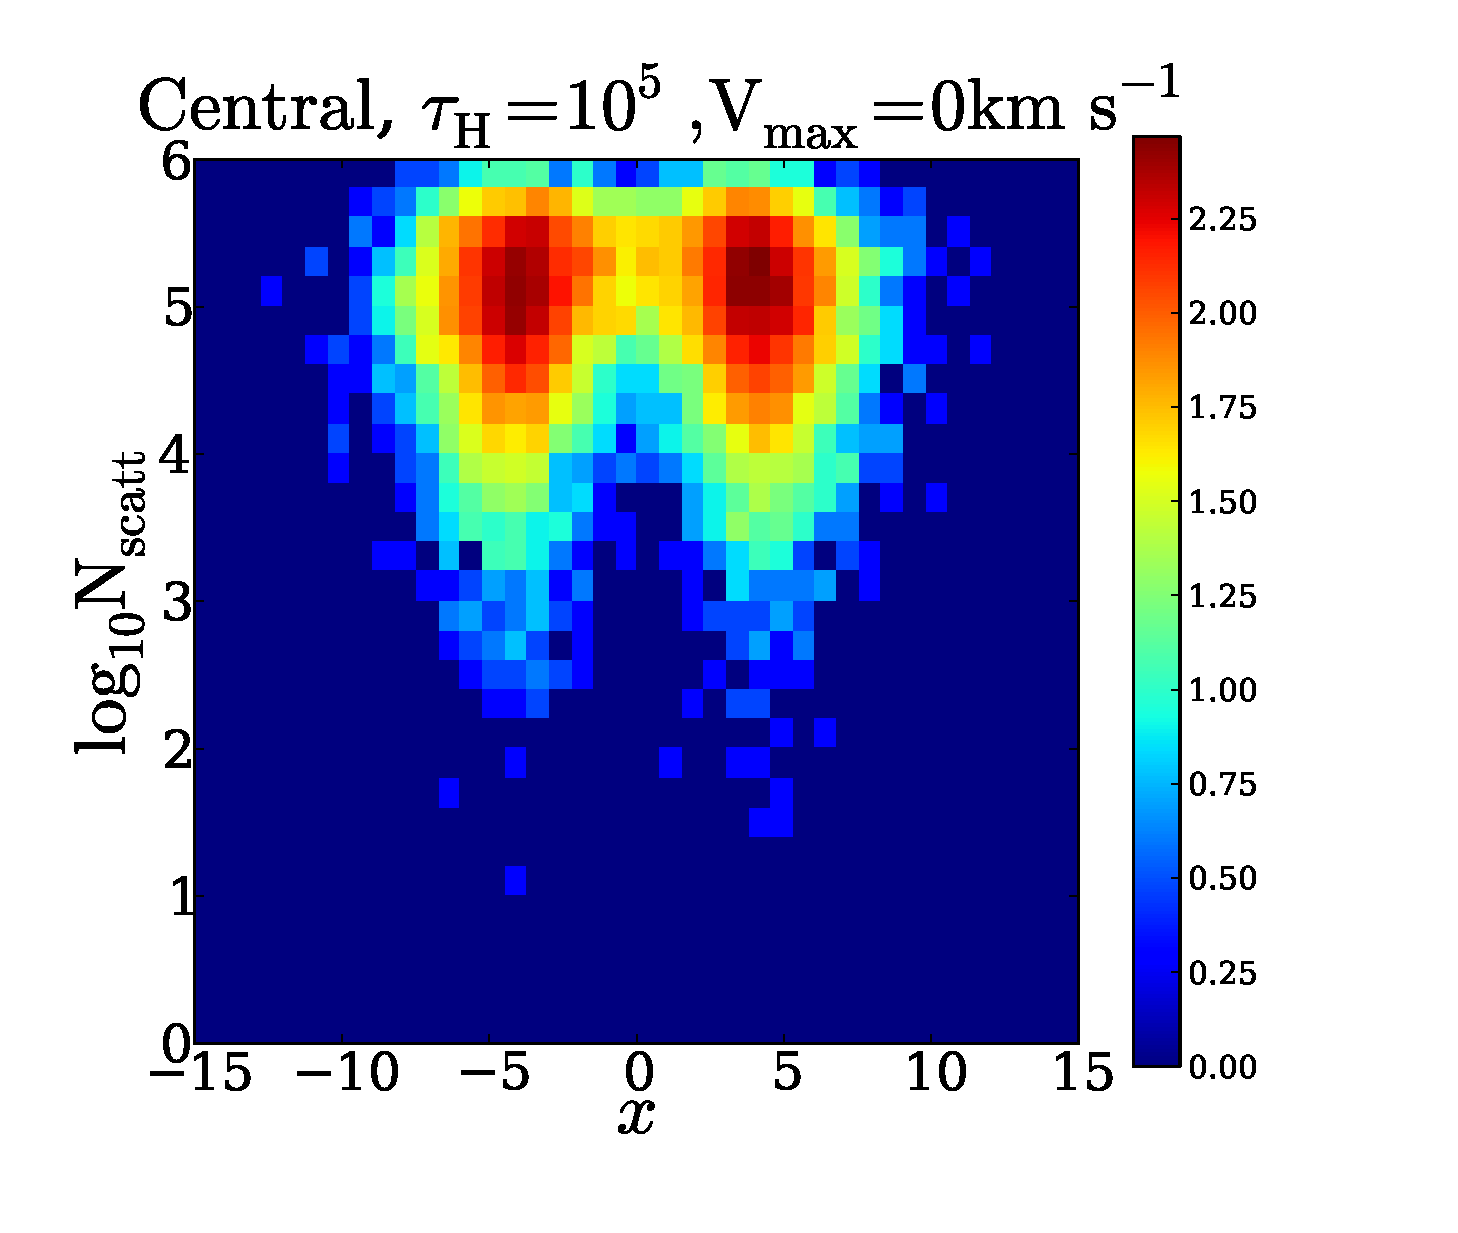
\includegraphics[width=0.48\textwidth]{f5_3.eps}
  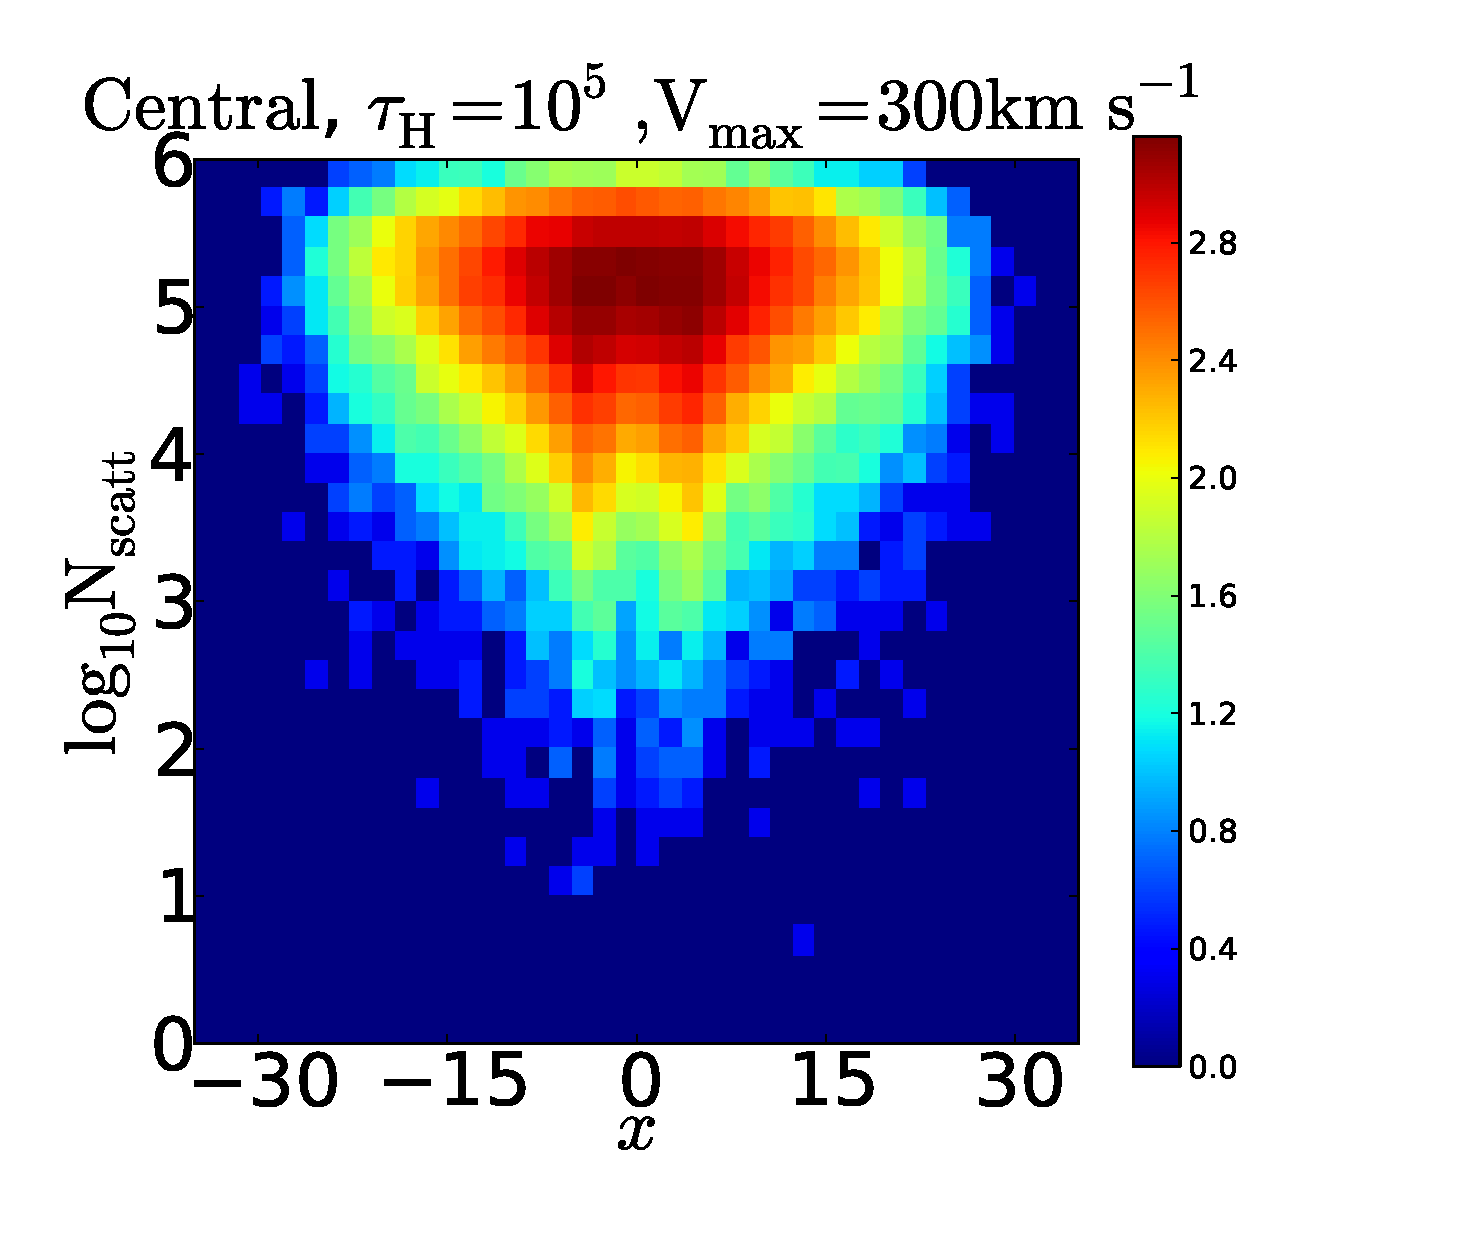
\includegraphics[width=0.48\textwidth]{f5_4.eps}    
\end{center}
    \caption{2D histogram of $N_{\rm scatt}$ vs $x$. The upper (lower) panels
      show the homogeneous (central) source distribution. Left panels 
      corresponds to the static case and right panels correspond to
      $V_{\rm max}=300\kms$. The color scale is logarithmic on the
      number of photons with given values of $N_{\rm scatt}$ and
      $x$. \label{fig:Nscatt2D}}   
\end{figure*}

%% One possible explanation for the emergence of the single peak in the
%% homogeneous systems is that some photons close to the surface
%% (a sort of photosphere) can escape with a low number of scatterings,
%% allowing them to stay close to the line's center. Increasing the
%% rotational velocity $V_{\rm max}$ reduces the optical depth making the
%% photosphere region effectively larger, increasing the number of
%% photons escaping close to the line's center. 

%% However, for the central emission the transition to a single peak is
%% harder to reach in the range of explored parameters. 
%% In this case the average number of scatterings to escape
%% should remain close to constant as the rotational velocity
%% increases. The rise in intensity at the line's center could instead
%% mean that the scattering in a medium with bulk motion are inefficient
%% in driving photons outside that frequency region.

%% In order to explore our interpretation for these two scenarios we now 
%% quantify the effect of rotation on the number of scatterings.


The number of scatterings affects the escape frequency of a \ly
photon. Studying this quantity can help us in claryfying two results
that we have observed for homogeneous models in the previous sections:
the quick emergence of a single peak and the increase in the escape
fraction.

A possible explanation for these two results is that some photons
close to the surface can escape with a low number of scatterings. This
has a two-fold consequence: the escaping photons do not have time to
scatter away from the line's center and also have less chances to find
an absorbing dust grain.


In Figure \ref{fig:Nscatt} we show the average number of scatterings
$\langle N_{\rm scatt}\rangle$ as a function of the cosinus of the
outgoing angle $|\cos\theta|$ and the rotational velocity
$V_{\rm max}$. From the right panel observe that the number of
scatterings and the outgoing angle are independent. This plot
corresponds to the specific case of the central model with $\tau=10^5$ and
$V_{\rm max}=300$\kms; but we have veryfied that this holds for all
models. This allows us to focus to use all the photons in the
simulations regardless of their value of $\cos\theta$. 

In the right panel of Figure \ref{fig:Nscatt} we observe how the
average number of scatterings decreases for larger rotational
velocities in the case of homogeneous source distributions. For instance, for
$\tau_{\rm H}=10^5$ the average number of scatterings decreases by
$61\%$ at $V_{\rm max}=300\kms$ in comparison to the static case. For
the central source distribution the average number of scatterings
$\langle N_{\rm   scatt}\rangle$ changes less than $0.5\%$. 


In static cases, a large value of the optical depth correlates with a
high number of scatterings.  This can be precisely quantified in the
static slab. In this model for centrally emitted sources the average
number of scatterings depends only on the optical depth $\langle
N_{\rm  scatt}\rangle=1.612\tau_{\rm   H}$
\citep{Adams72,Harrington73}, in the case of homogeneously distributed
sources $\langle N_{\rm   scatt}\rangle=1.16\tau_{\rm   H}$
\citep{Harrington73}.     

We perform a similar quantification of in our speherical setup for the
scatic spheres. We find that for the central model the number of
scatterings is proportional to the optical depth, with $\langle N_{\rm
  scatt}\rangle= (1.50, 1.00, 0.92)\tau_{\rm   H}$ for optical depth
values of $\tau_{\rm H} = (10^{5}, 10^{6}, 10^{7})$ respectively.
For the homogeneous static sphere we find that $\langle N_{\rm
  scatt}\rangle= (0.99, 0.59, 0.51)\tau_{\rm   H}$, this represents
factors of $(0.66, 0.59, 0.55)$ lower than the centrally  emitted photons. 

For the homogeneous rotating sphere at  $V_{\rm{max}}=300\kms$ we find
that $\langle N_{\rm   scatt}\rangle=(0.38, 0.34, 0.42)\tau_{\rm   H}$
which represents   factors of $(0.26, 0.34, 0.46)$ lower than the
corresponding central case.  

In order to gain a deeper understanding of these results  we make 2D
histograms for the number of scatterings as a function of the outgoing
dimensionless frequency $x$. In Figure \ref{fig:Nscatt2D} we these 
results in the case $\tau_{\rm H}=10^5$ for the
static case and $V_{\rm max}=300$\kms. The upper (lower) panels show the
results for the homogeneous (central) source distribution. The color
scale is logarithmic in the number of photons at a certain value
$x-N_{\rm scatt}$. 

The top right panel of Figure \ref{fig:Nscatt2D} (homogeneous sources,
high rotational velocity) supports our hypothesis about
the photo-sphere in the homogeneous distribution. In this case most of
the photons that left with $x\sim 0$ have escaped with less than $10$
scatterings. This also explains the decrease in the average number of
scatterings observed in Figure \ref{fig:Nscatt}.

However, for a central distribution the situation is quite different
(lower panels). In this case the number of scatterings remains high,
in the order of the optical depth, but the two peaks do get closer to each
other. Here the most probable physical picture is that each
scattering, due to the bulk velocity of the gas, is inefficient in
driving the photon outside the line center.


\section{Discussion}
\label{sec:discussion}

Gas bulk rotation has a noticeable effect on the morphology of the
 \ly line. In this section we compare our findings to other
 computational results and discuss the implications of these finding
 in the interpretation of observational data.


\cite{Verhamme12} studied \ly using two high resolution simulations
of individual galaxies. The main purpose of the study was to asses the
impact of two different InterStellar Medium (ISM) prescriptions. However, each simulated
galaxy had a disc structure with a clear rotation pattern in the ISM
and inflowing gas int the circum-galactic region. The configuration
had an axial symmetry and they reported a strong dependence of the
escape fraction and the total line intensity as a function of the
$\theta$ angle. In our results, none of these two quantities has a
dependence either on the inclination angle or the rotational
velocity. Therefore, the effect reported by \cite{Verhamme12} is
consistent with being a consequence of the different hydrogen optical
depth for different viewing angles and not as an effect of the bulk
rotation.  

The presence of single peaked profiles has been associated to
inflow/outflow dynamics \citep{Verhamme06,DijkstraKramer}. In this
paper we show that gas bulk rotation can also be considered as a
probable origin for that behavior, provided that the observed single peak is highly
symmetric. Similarly, in the case of double peaked lines with a high
level of flux at the line center, rotation also deserves to be considered in
the pool of possible bulk flows responsible for that feature,
specially if the two peaks have similar intensities. This highlights
that in order to interpret the observations of \ly emitting galaxies
it is necessary to consider the possible effect of different
inclination angles along the line of sight.


\section{Conclusions}
\label{sec:conclusions}

This paper quantifies for the first time in the literature the effects
of gas rotation in the morphology of the \ly emission line in star forming
galaxies.  The results are based on the study of an homogeneous sphere
of gas with solid body rotation. We explore a range of models by varying
the rotational speed, hydrogen optical depth, dust optical depth and
initial distribution of \ly photons with respect to the gas
density. As a cross-validation, we obtain our results from two
independently developed Monte-Carlo radiative transfer codes. 

Our main result is two-fold. First,rotation clearly impacts the \ly line
morphology. Second, rotation introduces an anisotropy for different
viewing angles. For viewing angles close to the poles the line is
double peaked and it makes a transition to a single peaked line for
high rotational velocities and viewing angles along the equator. This
trend is stronger for spheres with homogeneusly distributed radiation
sources.  In contrast, the total flux in the line remains independent
of the viewing angle.  


The escape fraction remains constant for diffenret viewing angles only
in the case of centrally distributed sources. In contrast, for an homogeneous
distribution the escape fraction decreases with high rotation 
fraction remain constant for different viewing angles. We showed that
these results can be interpreted in terms of the average number of
scatterings for the photons, a quantity that also remains constant
independent of the viewing angle and the rotational velocity for
centrally distributed sources and decreases for homogenously
distributed source.


Quantitatively the main results of our study are summarized as
follows. 

\begin{itemize}

\item Rotation induces a considerable asymmetry in the morphology 
 of the spectra when the viewing angle $\theta$. This occurs for
 all of our models. The asymmetry is such that observeds with
 $\cos\theta\equiv \mu\sim 1$, i.e. observes aligned with the rotation
 axis, the line is double peaked while for $\mu\sim 0$ and high
 rotation veolcities the linebecomes double peaked.

\item For $\mu \sim 0$ The line width increases with rotational velocity. The line width
  approximately follows the functional for  ${\rm FWHM}^2 = {\rm FWHM}_{
    0}^2 + (V_{\rm max}/\lambda)^2$ where FWHM$_{0}$ indicates the line
  width for the static case and $\lambda$ is a constant determined from
  the radiative transfer results it is $\lambda_{\rm c}=0.84 \pm 0.06$ and
  $\lambda_{\rm h}=0.54\pm 0.10$ for the central and homogeneous source
  distribution, respectively.

\item A single peaked line emerges for high rotational velocities in
  the case of homogeneously distributed sources. These cases occur when
  the rotational velocity is larger than half FWHM$_0$ and $\mu\sim 1$.  

\item 
For central sources we find that the escape fraction does not change
with rotational velocity nor with the viewing angle. We interpret this
in terms of the average number of scatterings which does not
significantly changes with rotation. This is due to the  
  fact that the vast majority of scatterings events are resonant, 
  during which the mean free path is very short and the effect of gas
  bulk rotation is not enough to affect \ly photons. 
  
\item For homogeneous sources we find that the  as rotational velocity
  increases, the escape fraction rises by a factor of $\sim 2$ with
  respect to the static situation. We also interpret this change in
  terms of the average number of scatterings. In the second part of \S
  \ref{sec:widthpeak} we show that the average number of scatterings
  decreases a $40\%$ compared to the static case, while a large
  fraction of photons escape with less than $10$ scatterings.  


\end{itemize}

Comparing our results with recent observed LAEs we find that many 
morphological features such as high central line flux, single peak
profiles  could be explained by gas bulk  rotation present in these
LAEs.  

\section*{Acknowledgments}

JNGC acknowledges financial support from Universidad de los
Andes. 

JEFR acknowledges financial support from Vicerrectoria de
Investigaciones at Universidad de los Andes through a FAPA grant.

We thank the International Summer School on AstroComputing
2012 organized by the University of California High-Performance
AstroComputing Center (UC-HiPACC) for providing computational
resources where some of the calculations were done. 

The data, source code and instructions to
replicate the results of this paper can be found
here {\texttt{https://github.com/jngaravitoc/RotationLyAlpha}}.
Most of our code benefits from the work of the IPython and Matplotlib
communities \citep{IPython,matplotlib}.




\bibliographystyle{apj}
\bibliography{references} 


\end{document}


